\documentclass[10pt,oneside,swedish]{article}
\usepackage{lmodern}
\usepackage{float}
\usepackage{amssymb,amsmath}
\usepackage{ifxetex,ifluatex}
\usepackage{fixltx2e} % provides \textsubscript
\ifnum 0\ifxetex 1\fi\ifluatex 1\fi=0 % if pdftex
  \usepackage[T1]{fontenc}
  \usepackage[utf8]{inputenc}
\else % if luatex or xelatex
  \ifxetex
    \usepackage{mathspec}
  \else
    \usepackage{fontspec}
  \fi
  \defaultfontfeatures{Ligatures=TeX,Scale=MatchLowercase}
\fi
% use upquote if available, for straight quotes in verbatim environments
\IfFileExists{upquote.sty}{\usepackage{upquote}}{}
% use microtype if available
\IfFileExists{microtype.sty}{%
\usepackage{microtype}
\UseMicrotypeSet[protrusion]{basicmath} % disable protrusion for tt fonts
}{}
\usepackage[unicode=true]{hyperref}
\hypersetup{
            pdftitle={ENVISIoN teknisk dokumentation},
            pdfborder={0 0 0},
            breaklinks=true}
\urlstyle{same}  % don't use monospace font for urls
\usepackage{graphicx,grffile}
\makeatletter
\def\maxwidth{\ifdim\Gin@nat@width>\linewidth\linewidth\else\Gin@nat@width\fi}
\def\maxheight{\ifdim\Gin@nat@height>\textheight\textheight\else\Gin@nat@height\fi}
\makeatother
% Scale images if necessary, so that they will not overflow the page
% margins by default, and it is still possible to overwrite the defaults
% using explicit options in \includegraphics[width, height, ...]{}
\setkeys{Gin}{width=\maxwidth,height=\maxheight,keepaspectratio}
\IfFileExists{parskip.sty}{%
\usepackage{parskip}
}{% else
\setlength{\parindent}{0pt}
\setlength{\parskip}{6pt plus 2pt minus 1pt}
}
\setlength{\emergencystretch}{3em}  % prevent overfull lines
\providecommand{\tightlist}{%
  \setlength{\itemsep}{0pt}\setlength{\parskip}{0pt}}
\setcounter{secnumdepth}{3}
% Redefines (sub)paragraphs to behave more like sections
\ifx\paragraph\undefined\else
\let\oldparagraph\paragraph
\renewcommand{\paragraph}[1]{\oldparagraph{#1}\mbox{}}
\fi
\ifx\subparagraph\undefined\else
\let\oldsubparagraph\subparagraph
\renewcommand{\subparagraph}[1]{\oldsubparagraph{#1}\mbox{}}
\renewcommand{\figurename}{Figur}
\fi

\title{ENVISIoN teknisk dokumentation}
\date{}

\begin{document}
\maketitle

© 2017 - Josef Adamsson, Robert Cranston, David Hartman, Denise
Härnström, Fredrik Segerhammar. \emph{(Teknisk dokumentation - release
1)}\\
© 2018 - Anders Rehult, Andreas Kempe, Marian Brännvall, Viktor
Bernholtz. \emph{(Teknisk dokumentation - release 2)}\\
© 2019 - Linda Le, Abdullatif Ismail, Anton Hjert, Lloyd Kizito and
Jesper Ericsson. \emph{(Teknisk dokumentation - release 3)}\\
© 2020 - Alexander Vevstad, Amanda Aasa, Amanda Svennblad, Daniel
Thomas, Lina Larsson and Olav Berg. \emph{(Teknisk dokumentation -
release 4)}\\
© 2017 - 2019 - Rickard Armiento, Johan Jönsson\\
© 2020 - Rickard Armiento, Joel Davidsson\\
© 2021 - Gabriel Anderberg, Didrik Axén, Adam Engman, Kristoffer Gubberrud Maras and Joakim Stenborg \emph{(Teknisk dokumentation - release 5)}

\newpage
\tableofcontents

\newpage
\section{Bakgrund}\label{bakgrund}

Elektronstrukturberäkningar är ett viktigt verktyg inom teoretisk fysik
för att förstå hur materials och molekylers egenskaper kan härledas från
kvantmekaniska effekter. För att förstå dessa egenskaper är det viktigt
att kunna analysera data från beräkningarna, något som förenklas och
görs möjligt genom visualisering. ENVISIoN är en kraftfull mjukvara som
är avsedd för visualisering av data från beräkningsprogram som VASP.
Mjukvaran bygger på forskningsverktyget Inviwo, utvecklad av
Visualiseringscenter i Norrköping. Idén med ENVISIoN är att underlätta
visualiseringarna från kvantmekaniska beräkningar. Det ska vara enkelt
och smidigt att visualisera önskade och relevanta egenskaper hos olika
system bestående av atomer. Mjukvaran tillgängliggör olika reglage och
knappar för att på ett interaktivt sätt kunna ändra dess egenskaper. I
följande dokument kommer de tekniska aspekterna av hur systemet är
implementerat att redovisas.

\subsection{Definitioner}\label{definitioner}

\begin{itemize}
\item
  \textbf{Inviwo:} Ett forskningsverktyg som utvecklas vid Linköpings
  universitet och ger användaren möjlighet att styra visualisering med
  hjälp av programmering i Python3 eller grafiskt. Det tillhandahåller
  även användargränssnitt för interaktiv visualisering \cite{Inviwo}.
\item
  \textbf{Processor:} Benämningen på ett funktionsblock i Inviwos
  nätverksredigerare som tar emot indata och producerar utdata. I detta
  dokument avser en processor alltid en inviwoprocessor om inte annat
  anges.
\item
  \textbf{Canvas:} En processor i Inviwo som ritar upp en bild i ett
  fönster.
\item
  \textbf{Data frame:} En tabell med lagrad data i form av tal. Varje
  kolumn i tabellen har ett specifikt namn.
\item
  \textbf{Transferfunktion:} Begrepp inom volymrendering för den
  funktion som används för att översätta volymdensiteter till en färg.
\item
  \textbf{Transferfunktionspunkt:} Ett värde i transferfunktionen som
  definerar en färg vid ett speciellt densitetsvärde.
\item
  \textbf{Port:} Kanal som processorer använder för att utbyta data av
  specifika typer.
\item
  \textbf{Property:} En inställning i en Inviwoprocessor.
\item
  \textbf{Länkar:} Kanaler som processorer använder för att länka samman
  properties av samma typ så att deras tillstånd synkroniseras.
\item
  \textbf{Nätverk:} Ett antal processorer sammankopplade via portar och
  länkar.
\item
  \textbf{Volymdata:} Tredimensionell data som beskriver en volym.
\item
  \textbf{API:} Application Programming Interface, en specifikation av
  hur olika applikationer kan användas och kommunicera med en specifik
  programvara. Detta utgörs oftast av ett dynamiskt länkat bibliotek
  \cite{API}. 
\item
  \textbf{BSD2:} En licens för öppen källkod \cite{BSD2}.
\item
  \textbf{C++:} Ett programmeringsspråk \cite{Cpp}. I Inviwo används
  C++ för att skriva programkod till processorer.
\item
  \textbf{Python3:} Ett programmeringsspråk \cite{Python}
  \cite{Python3}. I Inviwo används Python3 för att knyta samman
  processorer.
\item
  \textbf{Fermienergi:} Energinivån där antalet tillstånd som har en
  energi lägre än Fermienergin är lika med antalet elektroner i systemet
  \cite{Fermi-energi}.
\item
  \textbf{Git}: Ett decentraliserat versionshanteringssystem
  \cite{Git}.
\item
  \textbf{GUI:} (Graphical User Interface) Ett grafiskt
  användargränssnitt \cite{GUI}.
\item
  \textbf{PyQT:} En python-modul för GUI-programmering \cite{PyQT}.
\item
  \textbf{wxPython:} En samling av python-moduler för GUI-programmering
  \cite{wxPython}.
\item
  \textbf{PKF} En förkortning på Parkorrelationsfunktionen. Vilket
  ibland slarvigt kan anges synonymt som RDF, Radial Distribution
  Function \cite{RadialDistributionFunction}.
\item
  \textbf{HDF5:} Ett filformat som kan hantera stora mängder data. Alla
  HDF5-objekt har en rotgrupp som äger alla andra objekt i
  datastrukturen. Denna grupp innehåller i sin tur all övrig data i form
  av andra grupper, länkar till andra grupper eller dataset. Dataset
  innehåller rådata av något slag. Rådata kan i sammanhanget vara
  bilder, utdata från beräkningar, programdata, etc. \cite{HDFGroup}\cite{HDFGroup2}.

  De övriga objektstyperna gås inte igenom i detalj i detta dokument,
  men finns väl beskrivna i \emph{High Level Introduction to HDF5}
  \cite{HDFGroup2}.
\item
  \textbf{VASP:} The Vienna Ab initio simulation package, ett program
  för modellering på atomnivå, för t.ex. elektronstruktusrberäkningar
  och kvantmekanisk molekyldynamik \cite{VASP}.
\item
  \textbf{Parser:} Ett system som översätter en viss typ av filer till
  en annan typ av filer. I detta fall sker översättningen från
  textfiler, genererat i beräkningsprogrammet VASP, till HDF5-filer.
\item
  \textbf{Parsning:} Översättning utförd av parsern.
\item
  \textbf{Mesh} - Beskriver ett geometriskt objekt som en uppsättning av
  ändliga element.
\item
  \textbf{Array} - Ett dataobjekt som fungerar som behållare för element
  av samma typ \cite{WhatIsArray}.
\item
  \textbf{UNIX} - Benämning av en grupp operativsystem som härstammar
  från UNIX System from Bell Labs \cite{WhatIsUNIX}.
\item
     \textbf{Molekyldynamik} - Simuleringsmetod för att estimera atomers och molekylers rörelse. Vid simuleringen ges varje atom/molekyl ett startläge och en begynnelsehastighet. Därefter beräknas krafterna och accelerationen på atomerna/molekylerna. Slutligen genomförs ett tidssteg så att nya lägen och hastigheter fås och processen kan genomföras igen.   \cite{Molekyldynamik}
\item
    \textbf{Kraftvektor} - En tredimensionell vektor som visualiserar den kraft som påverkar ett objekt.

\end{itemize}

\newpage
\section{Översikt av systemet}\label{uxf6versikt-av-systemet}

\begin{figure}[H]
\centering
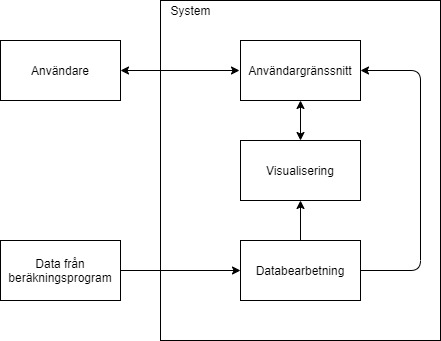
\includegraphics[width=1.00000\textwidth]{Images/system_overview.png}
\caption{Enkel skiss över systemet}
\label{fig:oversikt}
\end{figure}

Den produkt som utvecklas är ett verktyg för att visualisera viktiga
egenskaper från elektronstrukturberäkningar. Systemet skall bestå av ett
användargränssnitt där användaren får välja vilka beräkningsresultat som
skall konverteras och visualiseras.

I figur \ref{fig:oversikt} visas en grov systemskiss med de olika delsystem
som ingår. Systemet kan grovt delas upp i tre olika delar. Ett system
för databearbetning som parsar filer från VASP eller Elk, ett system för att
visualisera det som parsas i tidigare nämnt system, och ett GUI-system
vilket användaren interagerar med visualiseringen via.

\subsection{Ingående delsystem}\label{inguxe5ende-delsystem}

Systemet för elektronvisualisering består i huvudsak av tre delar. Dels
består systemet av en databearbetningsdel där parsning av textfiler
genererade från beräkningsprogrammet VASP skall översättas till det, med
vår mjukvara, kompatibla filformatet HDF5. Det går även att överföra filer från beräkningsprogrammet ELK till HDF5 filer.

När denna filkonvertering är klar så ska de genererade filerna behandlas
i ett visualiseringssystem för att skapa önskade visualiseringar.
Visualiseringen i Inviwo byggs upp av processorer vilka datan låts flöda
igenom för att skapa önskat slutresultat.

Den sista delen av systemet är det som möter användaren, det grafiska
användargränssnittet, GUI:t. Genom detta system skall tillgång till att
starta och göra ändringar i visualiseringen ges. Målet är att kunna
styra hela systemet från GUI:t som en fristående del från de två första
delsystemen.

\subsection{Ingående delsystem, mer
avancerat}\label{inguxe5ende-delsystem-mer-avancerat}

Detta kapitel beskriver översiktligt delsystemens relationer och
kommunikation med varandra. Det är menat som en sammanfattning av det
som kan läsas mer utförligt i kapitlen om de specifika systemen. För att
läsa detta rekomenderas en allafall grundläggande kunskap om hur inviwo
de olika delsystemen fungerar.

\begin{figure}[H]\label{}
\centering
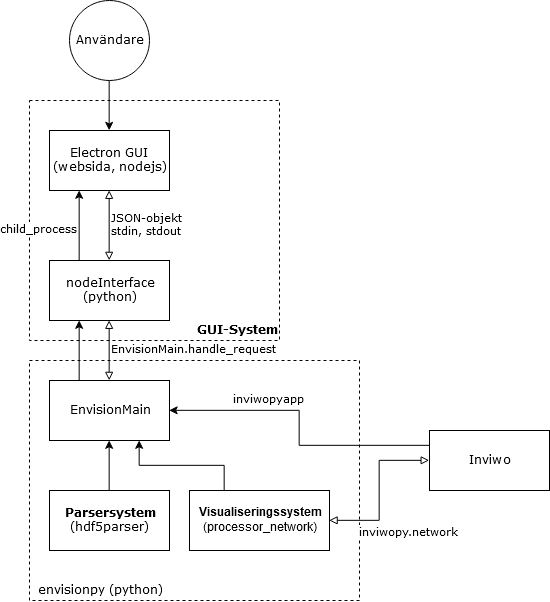
\includegraphics[width=1.00000\textwidth]{Images/Envision_system_advanced.png}
\caption{Skiss över delsystemens relationer till varandra.}
\end{figure}

Parsersystemet och visualiseringssystemet ingår i en pythonmodul kallad
\emph{envisionpy}. Se \ref{envisionpy} för mer detaljerad beskrivning. Denna
modul kan importeras från pythonskript för att få tillgång till
ENVISIoNs funktionalitet. Envisonpy har också en klass
\emph{EnvisionMain} (se \ref{envisionmain} för mer ingående). EnvisionMain
har som uppgift att vara ett gränssnitt där envisionpy kan styras från
ett utomliggande pythonskript. EnvisionMain initierar en instans av
Inviwo, genom pythonmodulerna inviwopyapp och inviwopy, som den kör i
bakggrunden. Detta gör att Inviwos funktioner kan användas utan att
Inviwos gränssnitt visas.

EnvisionMain-klassen har funktioner för att starta parsning genom att
köra funktioner från \emph{envisionpy.hdf5parser} (parsning beskrivet i \ref{parsersystemet}), och starta visualiseringar genom att initiera och
styra \emph{NetworkHandler}-klasser (se \ref{visualiseringssystemet},
\ref{networkhandlers}).

Gränssnittet är inte en del av envisionpy, utan är ett eget relativt
isolerat system. Gränssnittet bygger på electron och nodejs och är
skrivet med HTML, CSS, och JavaScript. Se \ref{gui-systemet} för mer
detaljerad information.

När systemet startas så laddas först den websida som är gränssnittet som
användaren ser. Från JavaScript-koden startas sedan, med hjälp av
node-modulen child\_process, en pythonprocess som kör skriptet
\emph{nodeInterface.py}. Detta skript initerar ett
\emph{EnvisionMain}-objekt. Det tar också hand om kommunikation mellan
javascript och python-processerna. Javascript- och pythonprocesserna
kommunicerar med varandra genom att läsa och skriva JSON-object i
pythonprocessens \emph{stdin} och \emph{stdout}.

Gränssnittet kan alltså nu begära att \emph{EnvisionMain} ska utföra
olika funktioner genom att skicka JSON-paket till den pythonprocess som
startats.

\newpage
\section{Parsersystemet}\label{parsersystemet}

Parserystemets uppgift är att omvandla information från VASP-filer till
data i HDF5-format, som visualiseringssystemet kan använda.
Parsersystemet är det delsystem i ENVISIoN som ser till att avläsa
korrekt data från VASP-filer och spara denna data i en lämplig
HDF5-filstruktur. Följande kapitel beskriver hur parsersystmet har
implementerats, samt redogör bakgrundskunskaper om HDF5, VASP och ELK.

Parsersystemet är implementerat i pythonkod och ligger under
envisionpy-modulen i envitionpy.hdf5parser.

\subsection{Bakgrundskunskap}\label{bakgrundskunskap}

För förståelse över hur parsersystemet implementerats krävs det lite
bakgrundskunskaper om hur HDF5 är uppbyggt och vad VASP är.

\subsubsection{VASP}\label{vasp}

VASP är ett beräkningsprogam som använder sig av Hartree-Fock metoden
eller täthetsfunktionalteori (DFT) för att approximera en lösning för
Schrödingerekvationen för mångpartikelfallet \cite{QuickStartGuide}.
VASP-filer kan delas upp i indatafiler och utdatafiler. I indatafiler
anges information som användaren kan manipulera, dessa indatafiler styr
hur beräkningarna ska utföras. Efter beräkningar genereras sedan ett
antal utdatafiler som innehåller kalkylresultaterna. Varje datafil
korresponderar till specifik information om systemet. Nedan återfinns
några viktiga VASP-filer.

\textbf{Utdatafiler:}

\begin{itemize}
\tightlist
\item
  CHG innehåller data om laddningstäthet.
\item
  DOSCAR innehåller data om tillståndstäthet.
\item
  EIGENVAL innehåller data för alla energier för k-rummet.
\item
  OUTCAR innehåller alla utdata.
\item
  XDATCAR innehåller data om enhetscell, atompositioner för varje
  beräkningssteg och även atomstyp.
\item
  CONTCAR innehåller data som den återfunnen i POSCAR, men innehåller
  information om atompositioner uppdateras.
\item
  PCDAT Innehåller data för parkorrelationsfunktionen, PKF.
\end{itemize}

\textbf{Indatafiler:}

\begin{itemize}
\tightlist
\item
  KPOINTS innehåller information om k-parametrarnas koordinater och
  vikter, alternativt instruktioner om hur en k-punkts mesh genereras av
  VASP.
\item
  INCAR innehåller information, i form av flaggor över hur beräkningar
  ska ske.
\item
  POSCAR innehåller data om enhetcellen och atompositionering.
\item
  POTCAR innehåller data om atomtyper.
\end{itemize}

Vid exempelvis beräkning av PKF för Si i temperaturen 300K, specificeras
information om hur systemet ser ut i filer som POSCAR. Sedan kan
information om hur beräkningarna ska genomföras specificeras i
exempelvis INCAR eller POTCAR. Detta kan röra sig om hur många
iterationer som ska ske och i vilka avstånd PKF ska beräknas. Då kan
exempelvis flaggor som NPACO och APACO sättas i INCAR-filen. Där flaggan
NPACO specificerar hur många iterationer som sker och APACO bestämmer
det längsta avståndet som sista iteration ska ha.

Efter beräkningen genereras flera utdatafiler, däribland PCDAT, som
innehåller värdena av PKF. Utdatafilen, PCDAT, kan då ha följande
utseende:

\begin{figure}[H]\label{}
\centering
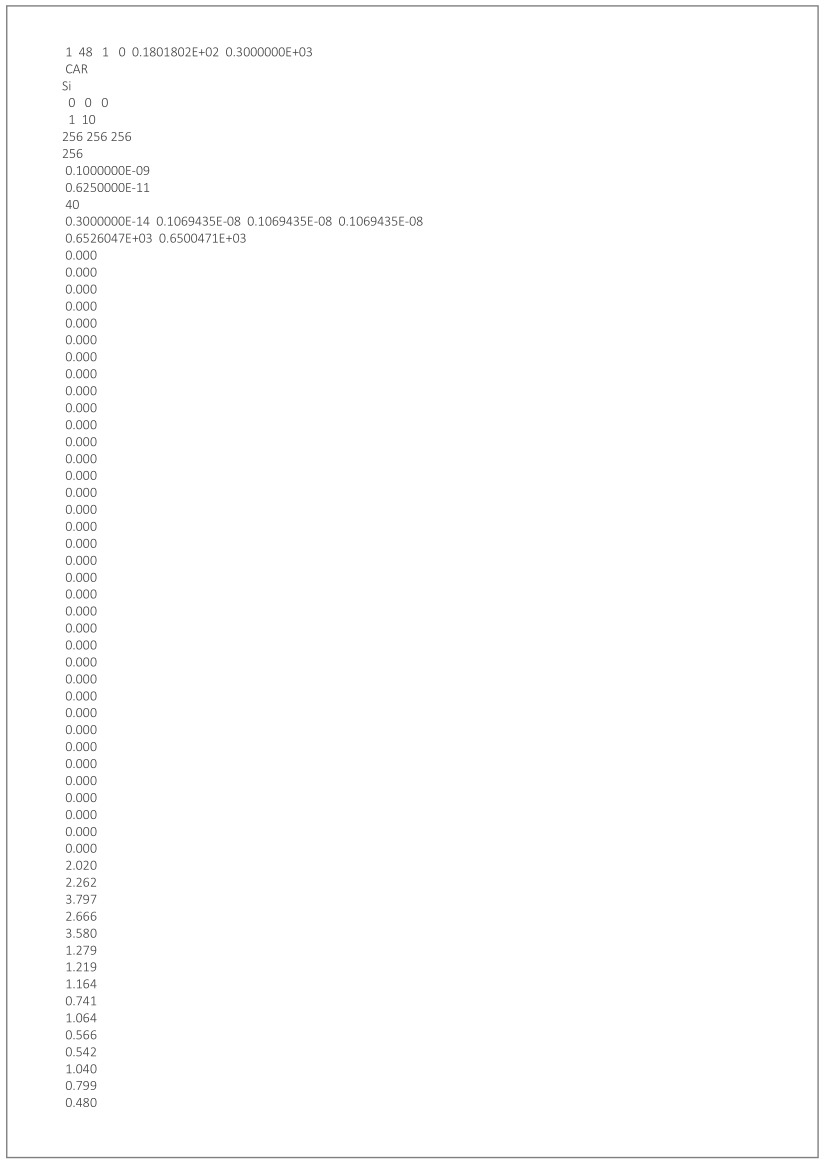
\includegraphics[width=1.00000\textwidth]{Images/PCDAT_utseende.png}
\caption{En demonstrativ bild över utseendet för PCDAT från VASP. Notera
att värdena inte riktigt stämmer.}
\end{figure}

Bilden ovan beskriver utseendet hos en del av PCDAT-filen för PKF för
systemet Si i 300K, med 40 olika tidsteg. Viktigaste är den långa
kolumnen av siffror som utgör definitionsmängden till funktionen.

\subsubsection{ELK}
 ELK är ett beräkningsprogramm som anvädner sig av full-potential linjär förstärkt-planvåg (FP-LAPW) kod för att lösa Schrödingerekvationen. På samma sätt som för VASP kan man dela upp ELK i indata och utdatafiler. Filerna har samma syfte för ELK som de har för VASP.

Till skillad från VASP så brukar ELK ofta ha en huvudinputfil, \textit{elk.in}. Efter \textit{elk.in} har körts i programmer så genereras det ett stort antal olika filer med ändelsen \textit{.OUT}. På samma sätt som för VASP så finns det en fil som innehåller mest data, \textit{INFO.OUT}.


\subsubsection{HDF5-format}\label{hdf5-format}

Vid hantering av stora mängder data, sådana genererade av
beräkningsprogram som VASP eller ELK, är HDF5-formatet mycket användbart. Det gör
specificiering av olika dataförhållanden och beroenden enkla, samt
tillgängliggör bearbetning av delar av data åt gången.

En HDF5-fil är ett objekt som innehåller en rotgrupp, som äger alla
andra grupper under den. Denna rotgrupp kan symboliseras av /.
Exempelvis /foo/zoo symboliserar \emph{zoo} som är en medlem till
\emph{group} \emph{foo}, som vidare är en medlem till rotgruppen. Ett
\emph{dataset} kan pekas av flera \emph{groups} \cite{HDFGroup2}.

\begin{figure}[H]\label{}
\centering
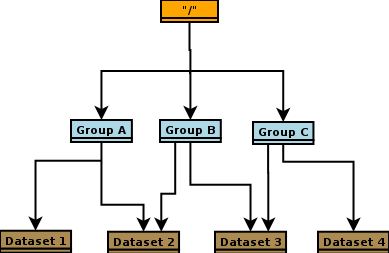
\includegraphics[width=1.00000\textwidth]{Images/DemonstrativHDF5bild.png}
\caption{Schematisk bild över HDF5 struktur}
\end{figure}

Mer ingående består \emph{dataset}-objektet av metadata och rådata.
Metadata beskriver rådatan, till den ingår \emph{dataspace},
\emph{datatype}, \emph{properties} och \emph{attributes}. Alla dessa är
HDF5-objekt som beskriver olika saker.

\emph{datatype} beskriver vad för datatyp varje individuell dataelement
i ett dataset har. Exempelvis kan detta vara ett 32-bitars heltal, eller
ett 32-bitars flyttal. I det mer komplexa fallet kan det också vara en
sammansättning av flera, vanligt benämnda, datatyper. \emph{Datatype}
beskriver då en följd av olika datatyper. Exempelvis en sammansättning
som int16, char, int32, 2x3x2 array av 32-bit floats beskriver att varje
dataelement i det gällande datasetet har en datatyp som består av 16
bitars heltal, en bokstav, 32-bitars heltal och slutligen en array av
flyttal med dimensionen 2x3x2. \emph{dataspace} är en HDF5-objekt som
beskriver hur datasetet sparar sin data, den kan exempelvis vara tom.
Ett dataset kan även bestå av ett enda tal, eller vara en array.
\emph{Properties} är mindre konkret än de två tidigare nämnda
egenskaperna och beskriver minneshanteringen av ett dataset. I dess
defaultläge exempelvist är dataset sparade kontinuerligt. Slutligen
återfinns HDF5-objektet \emph{attributes}, som kan valbart skapas.
Typiskt sätt skapas \emph{attributes} som ett sätt för att ytterligare
beskriva några egenskaper hos ett dataset. En \emph{attribute}
innehåller ett namn och ett värde, och skapas i samband med att ett
dataset öppnas \cite{HDFGroup2}.

\begin{figure}[H]\label{}
\centering
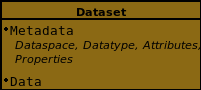
\includegraphics[width=0.50000\textwidth]{Images/Dataset_Metadata_HDF5.png}
\caption{Schematisk bild över \emph{dataset}.}
\end{figure}

ENVISIoN arbetar med HDF5-formatet. Python ger tillgång till hantering
av HDF5-formatet via paketet \emph{h5py}. Detta tillgängliggör
exempelvis läsandet av specifika element i massiva arrayer med
användandet av syntaxer tillgängliga av paketet \emph{numpy} \cite{HowToUseHDF5FilesinPython}.

Paketet \emph{h5py} ger upphov till HDF5-filer vilket kan ses som
behållare för två sorters objekt, \emph{datasets} och \emph{groups}.
\emph{datasets} är array-liknande ihopsättning av data, medan
\emph{groups} fungerar som behållare för andra \emph{groups} eller
\emph{datasets} \cite{HowToUseHDF5FilesinPython}. Elementen i
\emph{datasets} kan vara komplexa objekt. \emph{groups} kan återfinnas i
andra \emph{groups}, detta ger därmed möjlighet till konstruktion av
grupperingar av olika sammanhängande data. \emph{groups} och medlemmarna
till \emph{groups} fungerar som mappar och filer i UNIX. Varje
\emph{dataset} karaktäriseras exempelvis av en sökväg \cite{HDFGroup2}.

\subsection{ENVISIoNs HDF5-fil}\label{envisions-hdf5-fil}

ENVISIoNs parsersystem använder sig av pythonmodulen \emph{h5py} för att
generera en lämplig HDF5-filstruktur vid parsning. Den HDF5-strukturen
som genereras återfinns i nedstående diagram. Notera att figuren visas
som helbild i Appendix \ref{appendix-a---envisions-hdf5-filstruktur}.

\begin{figure}[H]
\centering
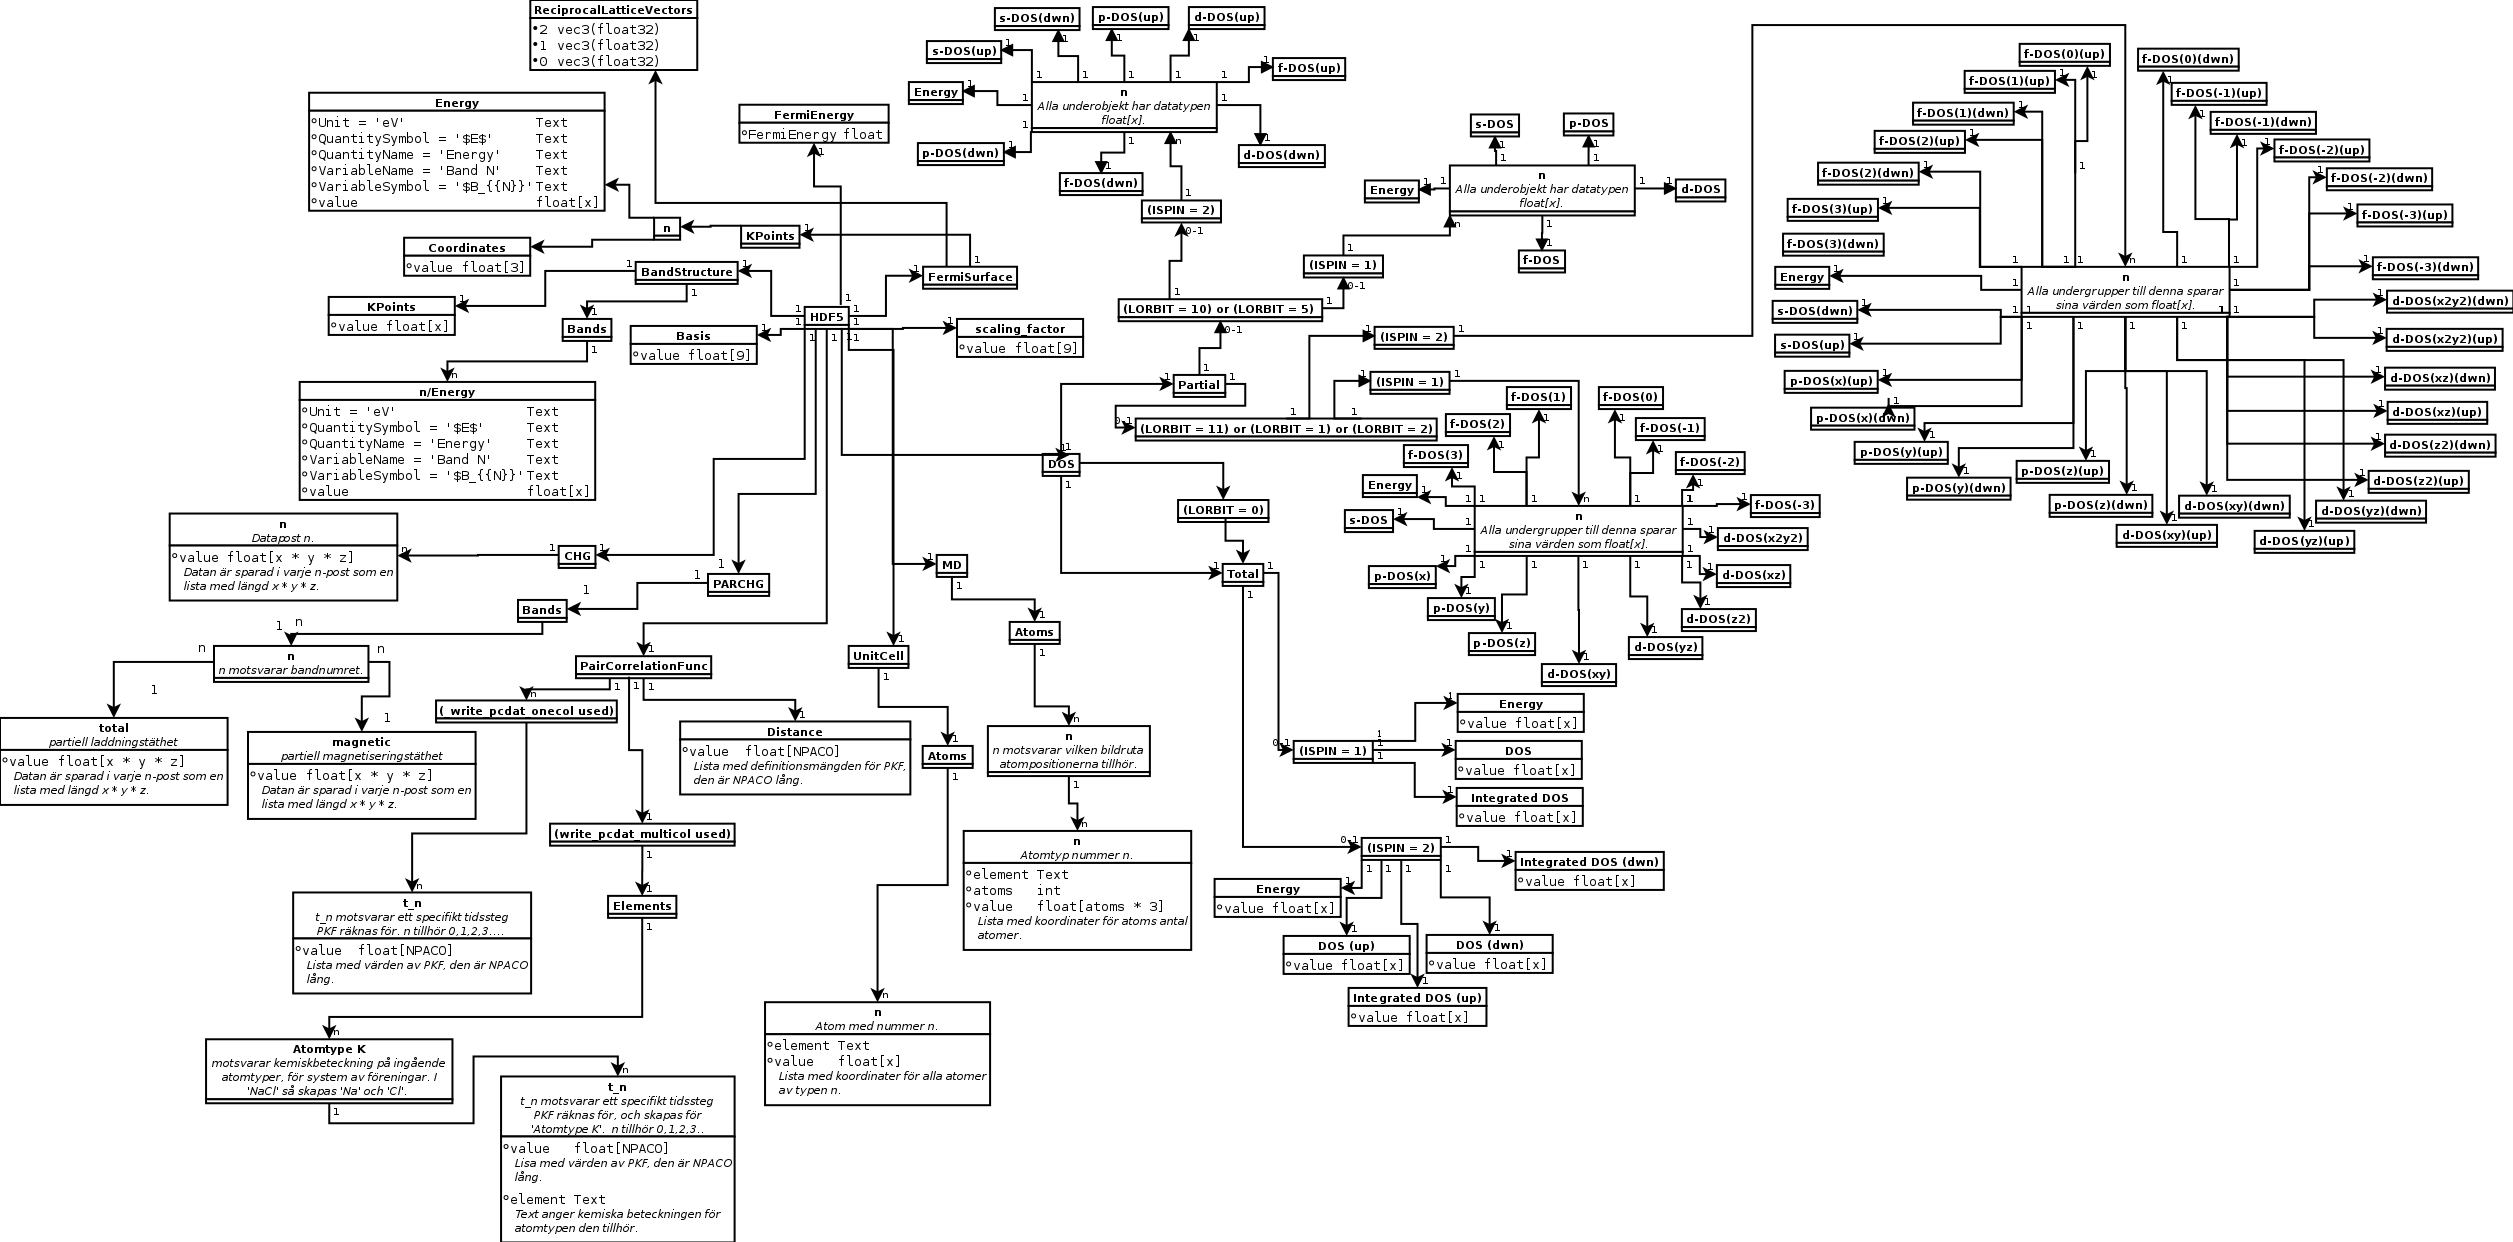
\includegraphics[width=1.00000\textwidth]{Images/UPDATE-hdf5-dataformat3modi.png}
\caption{En bild över HDF5-filstruktur som används i ENVISIoN.}
\label{fig:ENVISIoNsHDF5}
\end{figure}

I figur \ref{fig:ENVISIoNsHDF5} representeras olika grupper
(\emph{groups}) av lådor med pilar (förutom lådorna vars brödtext är
angiven i parantes), de sista lådorna i slutet av varje förgrening
representerar olika \emph{dataset}. Diagrammet beskriver alltså hur
information struktureras i en HDF5-fil som parsersystemet skapat. För
att få tillgång till ett visst \emph{dataset} måste en sökväg anges.
Denna sökväg är inget mer än en sträng bestående av olika grupper som
beskriver hur ett \emph{dataset} nås från rotgruppen, se under rubrik
sec:rotgruppstr\_. \ref{}

Varje \emph{dataset} kan bestå av ett antal olika fältnamn. Det fältnamn
som alltid förekommer är \emph{value}, vilket beskriver den huvudsakliga
datan som datasetet innehåller. Utöver det kan vissa andra fältnamn
också förekomma, exempelvis ``VariableName'' vilket är olika attribut,
\emph{attributes}, som beskriver andra egenskaper hos \emph{dataset} som
kan vara intressant.

Notera att diagram \ref{fig:ENVISIoNsHDF5} saknar viss information för DOS och för kraftvektorer.
DOS står för Density of States, översatt till tillståndstäthet. På grund
av platsbrist har inte attributen skrivits ut för DOS. p-DOS, d-DOS(xy),
Energy, grupper under DOS, med mera har attributen

\begin{itemize}
\tightlist
\item
  VariableName är fältets namn.
\item
  VariableSymbol är en symbol som representerar variabeln.
\item
  QuantityName är ett för en människa läsligt namn på fältet.
\item
  QuantitySymbol är symbol som representerar storheten.
\item
  Unit är storhetens fysikaliska enhet.
\end{itemize}

Kraftvektorer har samma struktur som unitcell har, förutom att \textit{value} anger både start- och slutpunkt för vektorn. 

Notera också att \emph{float{[}x{]}} avser en lista med längd x, samt
att alla grupper som är märkta med n är en metod att ange att det kan
finnas flera grupper på den nivån. Lådor vars rubrik är angivet inom
parentes anger ett villkor för att den resterande sökvägen ska kunna
skapas. Viktig anmärkning här är därför att dessa villkor inte ingår i
HDF5-strukturen, de är inga grupper, och ingår därmed inte med sökvägen
till de respektive dataseten. Under \emph{DOS} förekommer exempelvis en
sådan låda med brödtexten \emph{(LORBIT=0)}, samt under förgreningen hos
\emph{DOSPartial} förekommer en låda med angivelsen \emph{(ISPIN=0)}.
Båda \emph{ISPIN} och \emph{LORBIT} är flaggor som kan sättas i
INCAR-filen. I detta fall anger lådorna villkoren att \emph{(LORBIT=0)}
och \emph{(ISPIN=0)} för att den fortsatta respektive grupperna under
ska kunna skapas. Lådan under \emph{PairCorrelationFunc} anger dock
ingen sådan flagga. Det den anger är villkoret som har med huruvida
\emph{\_write\_pcdat\_onecol} eller \emph{\_write\_pcdat\_multicol}
används.

Parsning av PKF ges av olika möjligheter, parsern behandar en av
följande fall:

\begin{enumerate}
\tightlist
\item
  System av flera atomtyper, det som beräknas är en genomsnittlig PKF
  över alla atomtyper.
\item
  System av flera atomtyper, det som beräknas är en genomsnittlig PKF
  för varje atomtyp. Ingår det K atomtyper i systemet ska parsern ge
  upphov till K stycken parkorrelationsfunktioner.
\item
  System av 1 atomtyp.
\end{enumerate}

För fall 2 och 3 används \emph{\_write\_pcdat\_multicol} medan fall 1
använder \emph{\_write\_pcdat\_onecol}, se under \ref{skrivning-till-hdf5-fil}. Villkoren är därmed enbart ett sätt att ange
vad för fall parsern behandlar.

\subsection{Skrivning till HDF5-fil}\label{skrivning-till-hdf5-fil}

Det som skapar strukturen i HDF5-filen är skrivningsmodulen
\emph{h5writer} I ENVISIoN. \emph{h5writer.py} är ett skript som
innehåller alla skrivningsfunktioner som ingår i parsersystemet.
Funktionernas uppgift är att skapa \emph{datasets} (rådata) i rätt plats
i HDF5-fil objektet. Nedan listas alla funktioner som ingår i modulen.

\textbf{\_write\_coordinates} Denna funktion skriver koordinater för
atompositioner där varje atomslag tilldelas ett eget \emph{dataset}.
Attribut sätts för respektive grundämnesbeteckning per \emph{dataset}.

Parametrar:

\begin{itemize}
\tightlist
\item
  h5file: Sökväg till HDF5-fil, anges som en sträng.
\item
  atom\_count: Lista med antalet atomer av de olika atomslagen.
\item
  coordinates\_list: Lista med koordinater för samtliga atomer.
\item
  Elements: None eller lista med atomslag.
\end{itemize}

Returnerar:

\begin{itemize}
\tightlist
\item
  None
\end{itemize}

\textbf{\_write\_basis} Denna funktion skriver gittervektorerna i ett
dataset med namn basis.

Parametrar:

\begin{itemize}
\tightlist
\item
  h5file: Sökväg till HDF5-fil, anges som en sträng.
\item
  basis: Lista med basvektorerna.
\end{itemize}

Returnerar:

\begin{itemize}
\tightlist
\item
  None
\end{itemize}

\textbf{\_write\_scaling\_factor} Denna funktion skriver skalfaktorn för
gittret i ett dataset med namn scaling\_factor.

Parametrar:

\begin{itemize}
\tightlist
\item
  h5file: Sökväg till HDF5-fil, anges som en sträng.
\item
  scaling\_factor: Skalfaktorn för gittret.
\end{itemize}

Returnerar:

\begin{itemize}
\tightlist
\item
  None
\end{itemize}

\textbf{\_write\_fermi\_energy} Denna funktion skriver fermi-energin i
ett dataset med namn FermiEnergy.

Parametrar:

\begin{itemize}
\tightlist
\item
  h5file: Sökväg till HDF5-fil, anges som en sträng.
\item
  fermi\_energy: Fermi-energin för den aktuella uträkningen.
\end{itemize}

Returnerar:

\begin{itemize}
\tightlist
\item
  None
\end{itemize}

\textbf{\_write\_bandstruct} Denna funktion skriver ut data för
bandstruktur i en grupp med namn Bandstructure. Inom denna grupp
tilldelas specifika K-punkter, energier samt bandstrukturer egna
dataset. Högsymmetripunkter och deras symboler tilldelas egna dataset.
Diverse attribut sätts även för bl.a. specifika energier.

Parametrar:

\begin{itemize}
\tightlist
\item
  h5file: Sökväg till HDF5-fil, anges som en sträng.
\item
  band\_data: Lista med bandstrukturdata.
\item
  kval\_list: Lista med K-punkter för specifika bandstrukturdata.
\end{itemize}

Returnerar:

\begin{itemize}
\tightlist
\item
  None
\end{itemize}

\textbf{\_write\_dos} Denna funktion skriver ut DOS-data i en grupp med
namn DOS där total och partiell DOS tilldelas grupper med namn Total
respektive Partial. Inom gruppen Total tilldelas energin samt specifika
DOS egna dataset och inom gruppen Partial tilldelas varje partiell DOS
egna grupper där energin samt specifika DOS tilldelas egna dataset.

Parametrar:

\begin{itemize}
\tightlist
\item
  h5file: Sökväg till HDF5-fil, anges som en sträng.
\item
  total: En lista med strängar av de olika uträkningarna som har utförts
  av VASP för total DOS.
\item
  partial: En lista med strängar av de olika uträkningarna som har
  utförts av VASP för partiell DOS.
\item
  total\_data: En lista med alla beräkningar för total DOS för varje
  specifik atom.
\item
  partial\_list: En lista med alla beräkningar för partiell DOS för
  varje specifik atom.
\item
  fermi\_energy: Fermi-energin för den aktuella uträkningen.
\end{itemize}

Returnerar:

\begin{itemize}
\tightlist
\item
  None
\end{itemize}

\textbf{\_write\_volume} Denna funktion skriver ut elektrontäthetsdata
och elektronlokaliseringsfunktionsdata (ELF) till grupper med namn CHG
respektive ELF. Inom dessa grupper tilldelas varje iteration ett
dataset.

Parametrar:

\begin{itemize}
\tightlist
\item
  h5file: Sökväg till HDF5-fil, anges som en sträng.
\item
  i: Skalär som anger numret på iterationen.
\item
  partial: En lista med strängar av de olika uträkningarna som har
  utförts av VASP för partiell DOS.
\item
  array: Array med parsad data för respektive iteration.
\item
  data\_dim: Lista som anger dimensionen av data för respektive
  iteration.
\item
  hdfgroup: En textsträng med namnet på vad man vill kalla gruppen i
  HDF5-filen.
\end{itemize}

Returnerar:

\begin{itemize}
\tightlist
\item
  None
\end{itemize}

\textbf{\_write\_incar} Denna funktion skriver ut parsad data från INCAR
i ett dataset med namn Incar där varje datatyp tilldelas egna dataset.

Parametrar:

\begin{itemize}
\tightlist
\item
  h5file: Sökväg till HDF5-fil, anges som en sträng.
\item
  incar\_data: Datalexikon med all data från INCAR-filen.
\end{itemize}

Returnerar:

\begin{itemize}
\tightlist
\item
  None
\end{itemize}

\textbf{\_write\_pcdat\_onecol} Denna funktion skapar ett HDF5-struktur
för ett system med flera atomtyper, där en genomsnittlig PKF beräknas
för alla atomtyper. Funktionen skapar en HDF5-struktur som innehåller
data från huvudsakligen PCDAT.

Parametrar:

\begin{itemize}
\tightlist
\item
  h5file: Sökväg till HDF5-fil, anges som en sträng.
\item
  pcdat\_data: Tillhör Python-datatypen \emph{dictionary} \cite{dict}.
  Detta argument innehåller alla värden av PKF som parsats.
\item
  APACO\_val: Värdet på APACO-flaggan i VASP-filen INCAR eller POTCAR.
  Defaultvärde är 16 Ångström. Flaggan anger det längsta avståndet sista
  iteration för beräkning av PKF har.
\item
  NPACO\_val: Värdet på NPACO-flaggan i VASP-filen INCAR eller POTCAR.
  Defaultvärde är 256. Flaggan anger hur många iterationer ska ske för
  beräkning av PKF.
\end{itemize}

Returnerar:

\begin{itemize}
\tightlist
\item
  None
\end{itemize}

\textbf{\_write\_pcdat\_multicol} Denna funktion skapar ett
HDF5-struktur för ett system med flera atomtyper, där en genomsnittlig
PKF beräknas för varje atomtyp som ingår i systemet. Funktionen anropas
också i fallet då systemet enbart består av en atomtyp. Funktionen
skapar en HDF5-struktur som innehåller data från huvudsakligen PCDAT.

Parameterar:

\begin{itemize}
\tightlist
\item
  h5file: Sökväg till HDF5-fil, anges som en sträng.
\item
  pcdat\_data: Tillhör Python-datatypen \emph{dictionary} \cite{dict}.
  Detta argument innehåller alla värden av PKF som parsats.
\item
  APACO\_val: Värdet på APACO-flaggan i VASP-filen INCAR eller POTCAR.
  Defaultvärde är 16 Ångström. Flaggan anger det längsta avståndet sista
  iteration för beräkning av PKF har.
\item
  NPACO\_val: Värdet på NPACO-flaggan i VASP-filen INCAR eller POTCAR.
  Defaultvärde är 256. Flaggan anger hur många iterationer ska ske för
  beräkning av PKF.
\end{itemize}

Returnerar:

\begin{itemize}
\tightlist
\item
  None
\end{itemize}

\textbf{\_write\_force}
Denna funktion skapar ett HDF5-struktur för ett system där det finns krafter som verkar mellan atomerna. Funktionen skriver vektorernas start och slutpunkter till HDF5 där vektorernas startpunkt sammanfaller med atomens position.

Parameterar:

\begin{itemize}
\tightlist
\item
  h5file: Sökväg till HDF5-fil, anges som en sträng.
\item
  force\_list: Innehåller en lista över all vektorinformation för varje atom.
\item
  atom\_count: Antalet atomer som en int.
\end{itemize}

Returnerar:

\begin{itemize}
\tightlist
\item
  None
\end{itemize}

\textbf{\_write\_md} Denna funktion skriver ut data för molekyldynamik till en grupp med namn MD. Varje tidssteg placeras i gruppen MD i ett eget dataset.

Parametrar:
\begin{itemize}
\tightlist
\item h5file: Sökväg till HDF5-fil, anges som en sträng
\item atom\_count: lista med fördelningen i antal av de olika atomerna
\item cordinates\_list: lista med kordinaterna för varje atom i tidssteg
\item elements: lista över atomtyper 
\item step: nuvarande tidssteg
\end{itemize}
\subsection{Inläsning av VASP-filer}\label{inluxe4sning-av-vasp-filer}

Innan en funktion kan skriva till HDF5-objektet krävs det att rätt
inläsning av innehåll från relevant VASP-fil har skett. Detta är vad de
olika läsningsfunktionerna i parsersystemet gör. Typiskt återfinns en
pythonmodul för varje egenskap hos ett system som ska parsas. Nedan
listas alla sådana moduler.

\subsubsection{Bandstrukturparser}\label{bandstrukturparser}

Bandstrukturparsern läser in alla energier för k-parametrar från
EIGENVAL-filen i användarens VASP-mapp, som skrivs till /Bandstructure i
HDF5-filen och dessutom skrivs de inlästa k-parametrarnas koordinater
från EIGENVAL-filen in i /BandStructure i HDF5-filen.
Högsymmetripunkteroch dess symboler läses av från KPOINTS-filen och
Bravais-gittrets typ läses av från OUTCAR-filen i användarens VASP-mapp
och dessa punkter och tillhörande symboler skrivs in i egna datasets
under /Highcoordinates i HDF5-filen.

Funktionsanrop: envisionpy.hdf5parser.bandstructure(h5file, vasp\_dir)

Parameterar:

\begin{itemize}
\tightlist
\item
  h5file: Sökväg till HDF5-fil, anges som en sträng.
\item
  vasp\_dir: Sökväg till VASP-katalog, anges som en sträng.
\end{itemize}

Returnerar:

\begin{itemize}
\tightlist
\item
  Bool: True om parsning skett felfritt, False annars.
\end{itemize}

\subsubsection{Incarparser}\label{incarparser}

Incarparsern består av en pythonfil med namnet incar som innehåller
funktionerna, incar och parse\_incar. Dessa funktioner läser in och
sparar information från INCAR-filen samt anropar en separat pythonmodul
som skriver en HDF5-fil.

Funktionen incar kontrollerar att HDF5-filen redan innehåller INCAR-data
och anropar funktionen parse\_incar om så inte är fallet. Existerar
INCAR-filen i användarens VASP-katalog parsas data av funktionen
parse\_incar som då sparar ett dataset för varje datatyp och namnger
dataseten därefter. Funktionen incar anropar sedan pythonmodulen som
skriver HDF5-filen där varje enskilt \emph{dataset} tilldelas en egen
grupp.

Funktionsanrop: envisionpy.hdf5parser.incar(h5file, vasp\_dir)

Parameterar:

\begin{itemize}
\tightlist
\item
  h5file: Sökväg till HDF5-fil, anges som en sträng.
\item
  vasp\_dir: Sökväg till VASP-katalog, anges som en sträng.
\end{itemize}

Returnerar:

\begin{itemize}
\tightlist
\item
  Lista med namn på data (\emph{datasets}) som parsas.
\item
  Bool: True om parsning skett felfritt, False annars.
\end{itemize}

\subsubsection{Volymparser}\label{volymparser}

Volymparsern består av en mängd funktioner i en pythonfil som används
för parsning av CHG och ELFCAR. Den kan läsa in och spara data på
HDF5-format från båda dessa filer genom att anropa en pythonmodul. Detta
är för att CHG och ELFCAR har samma struktur och består av ett antal
iterationer av volymdata från volymberäkningar. Således innehåller den
sista iterationen data som är mest korrekt. Därför skapar volymparsern
också en länk till den sista iterationen i HDF5-filen för att data av
högst kvalitet lätt ska kunna plockas ut.

Funktionsanrop vid parsning av CHG-data:
envisionpy.hdf5parser.charge(h5file, vasp\_dir)

Funktionsanrop vid parsning av ELFCAR-data:
envisionpy.hdf5parser.elf(h5file, vasp\_dir)

Parameterar:

\begin{itemize}
\tightlist
\item
  h5file: Sökväg till HDF5-fil, anges som en sträng.
\item
  vasp\_dir: Sökväg till VASP-katalog.
\end{itemize}

Returnerar:

\begin{itemize}
\tightlist
\item
  Bool: True om parsning skett felfritt, False annars.
\end{itemize}

\subsubsection{Tillståndstäthetsparser}\label{tillstuxe5ndstuxe4thetsparser}

Tillståndstäthetsparsern består av en mängd funktioner i en pythonfil
som används för parsning av DOSCAR. DOSCAR-filen består först av den
totala tillståndstätheten och sedan partiell tillståndstäthet för varje
atom i kristallen. Beroende på vad som står i INCAR kan dock denna data
se väldigt olika ut. Flaggorna ISPIN, RWIGS och LORBIT i INCAR-filen
avgör vad som skrivs i DOSCAR-filen. ISPIN-flaggan informerar om spinn
har tagits hänsyn till vid beräkningar, RWIGS-flaggan specificerar
Wigner-Seitz-radien för varje atomtyp och LORBIT-flaggan (kombinerat med
RWIGS) avgör om PROCAR- eller PROOUT-filer (som DOSCAR-filen refererar
till) skrivs. Parsern läser därför från data givet av incarparsern i
HDF5-filen för att se hur DOSCAR ska parsas. Parsern delar upp data i
två grupper i HDF5-filen, total och partiell. I gruppen partiell finns
det en grupp för varje atom. Ett dataset för varje undersökt fenomen
skrivs sedan ut för varje atom under partiell, och för total
tillståndstäthet under total.

Funktionsanrop: envisionpy.hdf5parser.dos(h5file, vasp\_dir)

Parameterar:

\begin{itemize}
\tightlist
\item
  h5file: Sökväg till HDF5-fil, anges som en sträng.
\item
  vasp\_dir: Sökväg till VASP-katalog.
\end{itemize}

Returnerar:

\begin{itemize}
\tightlist
\item
  Bool: True om parsning skett felfritt, False annars.
\end{itemize}

\subsubsection{Enhetscellsparser}\label{enhetscellsparser}

Enhetscellparsern läser in gittervektorer, som multipliceras med
skalfaktorn och skrivs till /basis i HDF5-filen. Atompositioner läses
från POSCAR och om dessa är angivna med kartesiska koordinater räknas de
om till koordinater med gittervektorerna som bas. Koordinaterna skrivs
till HDF5-filen uppdelade efter atomslag och attribut sätts med
respektive grundämnesbeteckning. Om dessa inte ges med parametern
elements letar parsern i första hand i POTCAR och i andra hand i POSCAR.

Funktionsanrop: envisionpy.hdf5parser.unitcell(h5file, vasp\_dir,
elements = None)

Parameterar:

\begin{itemize}
\tightlist
\item
  h5file: Sökväg till HDF5-fil, anges som en sträng.
\item
  vasp\_dir: Sökväg till VASP-katalog.
\item
  elements = None: None eller lista med atomslag.
\end{itemize}

Returnerar:

\begin{itemize}
\tightlist
\item
  Bool: True om parsning skett felfritt, False annars.
\end{itemize}

\subsubsection{Parkorrelationsfunktionsparser}\label{parkorrelationsfunktionsparser}

Parkorrelationsfunktionsparser använder sig av ett antal olika
funktioner, vilka alla anropas med funktionen
\emph{paircorrelation(h5file, vasp\_dir)}. Parsningen görs genom
inläsning av korrekt data från PCDAT-filen, samt inläsning av flaggor
som NPACO och APACO. Parsen letar efter dessa flaggor i INCAR eller
POTCAR för att se om de är satta. I fallet de inte är det antas deras
defaultvärden.

Funktionsanrop: envisionpy.hdf5parser.paircorrelation(h5file, vasp\_dir)

Parameterar:

\begin{itemize}
\tightlist
\item
  h5file: Sökväg till HDF5-fil, anges som en sträng.
\item
  vasp\_dir: Sökväg till VASP-katalog.
\end{itemize}

Returnerar:

\begin{itemize}
\tightlist
\item
  Bool: True om parsning skett felfritt. Ett undantag kan kastas om
  PCDAT-fil inte hittas.
\end{itemize}

\subsubsection{Fermi-yta parser}\label{fermi-yta-parser}

Reads OUTCAR and EIGNVAL to create datastructure for visualization of
fermi surfaces

\begin{description}
\item[Parameters:]
\begin{description}
\item[hdf\_file\_path: str]
Path where hdf file will be written to
\item[vasp\_dir\_path: str]
Path of direcotry containing OUTCAR and EIGENVAL files
\end{description}
\item[Returns:]
True if succesfull else False
\end{description}

\subsubsection{Kraftparser}\label{Kraftparser}
Läser in data om vilka krafter som verkar på atomerna från OUTCAR och atomernas positioner från POSCAR för att ta fram relevant information om kraftvektorerna som tillhör de enskilda atomerna.

Funktionsanrop: envisionpy.hdf5parser.force\_parser(h5file, vasp\_dir, \\ inviwo = False)

Parameterar:

\begin{itemize}
\tightlist
\item
  h5file: Sökväg till HDF5-fil, anges som en sträng.
\item
  vasp\_dir: Sökväg till VASP-katalog.
\item
  inviwo = False: Ska sättas till True om körning sker från Inviwo
\end{itemize}

Returnerar:

\begin{itemize}
\tightlist
\item
  Bool: True om parsning skett felfritt, False annars.
\end{itemize}


\subsubsection{Molekyldynamikparser}\label{Molekyldynamikparser}
Molekyldynamikparser består av en mängd funktioner i en pythonfil som används för parsning av XDATCAR om molekyldynamik är möjligt. För att avgöra om molekyldynamik är möjligt granskas IBRION flaggan i OUTCAR filen. Om IBRION flag är satt till 0 är molekyldynamik ok. 

Funktionsanrop: envisionpy.hdf5parser.mol\_dynamic\_parser((hdf5\_file\_path, vasp\_dir\_path, element = None)

Parametrar:
\begin{itemize}
\tightlist
\item Sökväg till HDF5-fil, anges som en sträng.
\item Sökväg till VASP-katalog.
\item elements = None: None eller lista med atomslag.
\end{itemize}


\subsubsection{parse\_all}\label{parse_all}

parse\_all är en funktion för parsning av allt som finns i katalogen som
ges som inparameter. Funktionen kallar på alla systemets parsers och
skriver ut meddelande om vad som parsas och om parsningen gjordes eller
ej.

Funktionsanrop: envision.parse\_all(h5\_path, dir)


Parameterar:

\begin{itemize}
\tightlist
\item
  h5\_path: Sökväg till HDF5-fil, anges som en sträng.
\item
  vasp\_dir: Sökväg till katalog med utdata-filer från
  beräkningsprogram.
\end{itemize}

Returnerar:

\begin{itemize}
\tightlist
\item
  Bool: True om parsning skett felfritt, False annars.
\end{itemize}

\subsection{Inläsning av Elk-filer}
För att en funktion ska kunna skrivas till ett HDF5-objektet krävs det att rätt inläsning av innehåll från relevanta ELK-filer har skett. Detta sker via läsningsfunktionerna i parsersystemet. Typiskt återfinns en pythonmodul för varje egenskap som ska parsas. Nedan listas alla sådana moduler implementerade för ELK.

\subsubsection{Enhetscellparser}
Enhetscellparsern läser in gittervektorer, som multipliceras med skalfaktorn och skrivs till /basis i HDF5-filen. Atompositioner läses från INFO.OUT. Koordinaterna skrivs till HDF5-filen uppdelade efter atomslag och attribut sätts med respektive grundämnesbeteckning. Typ av atomslag och hur många av varje atomslag tas fram ur filen EQATOMS.OUT.

Funktionsanrop: envisionpy.hdf5parser.unitcell\_parser(h5file, ELK\_dir)

Parameterar:
\begin{itemize}
\tightlist
\item h5file: Sökväg till HDF5-fil, anges som en sträng.
\item ELK\_dir: Sökväg till ELK-katalog.
 
\end{itemize}

\subsubsection{Kraftparser}
Läser in data om vilka krafter som verkar på atomerna samt atomernas positioner från ELK filen INFO:OUT för att ta fram relevant information om kraftvektorerna som tillhör de enskilda atomerna. Typ av atomslag och hur många av varje atomslag tas fram ur filen EQATOMS.OUT.

Funktionsanrop: envisionpy.hdf5parser.parse\_force\_elk(h5file, elk\_dir, \\ inviwo = False, elements = None)

Parameterar:

\begin{itemize}
\tightlist
\item
  h5file: Sökväg till HDF5-fil, anges som en sträng.
\item
  elk\_dir: Sökväg till ELK-katalog.
\item
  inviwo = False: Ska sättas till True om körning sker från Inviwo
  
\item elements = None: None eller lista med atomslag.
\end{itemize}

Returnerar:

\begin{itemize}
\tightlist
\item
  Bool: True om parsning skett felfritt.
\end{itemize}
\subsubsection{ELF-parser}

Funktionsanrop:
envisionpy.hdf5parser.parse\_elf(h5file, ELK\_dir)

Parameterar:

\begin{itemize}
\tightlist
\item
  h5file: Sökväg till HDF5-fil, anges som en sträng.
\item
  ELK\_dir: Sökväg till ELK-katalog.
\end{itemize}

Returnerar:

\begin{itemize}
\tightlist
\item
  Bool: True om parsning skett felfritt.
\end{itemize}

\subsection{Testning}\label{testning}

För att varje års projekt ska kunna kontrollera att alla parsersystem
fungerar är det viktigt med testfiler. Detta kan också ge inblick i hur
parsern är tänkt att fungera. En generell testmapp i ENVISIONs
filstruktur för parsersystemet finns vid namn /unit\_testing. Mappen
innehåller tester för parsning av bandstrukturer, tillståndstätheter,
elektrontäthet, enhetscell, fermi-ytor, kraftvektorer och molekyldynamik. Testerna är skapade att testa
om HDF5-filer genereras ur parsersystemen och om de genererade
HDF5-filerna har korrekt datastruktur.

Test för exempelvis parsersystemet för bandstrukturer har implementerats
med en testfil med namnet \emph{test\_bandstructure\_parsing.py} samt en
mapp vid namn \emph{resources}. I \emph{resources} finns det olika
mappar med VASP-filer för olika kristaller, som därmed testar att
parsern fungerar korrekt för olika filer. Det är tanken att framtida
utvecklare använder sig av denna mapp för att lägga in tester för
nyskapade funktioner för parsning av någon ny egenskap. 

\newpage
\section{Visualiseringssystemet}\label{visualiseringssystemet}

Visualiseringssystemet är det delsystem som använder den HDF5-fil som
parsersystemet genererar för att visualisera beräkningsresultaten. Detta
görs genom olika nätverk, bestående av processorer. Nedstående kapitel
redovisar de olika befintliga nätverk ENVISIoN består av.

\subsection{Nätverk}\label{nuxe4tverk}

För att visualiseringssytemet ska vara kompatibelt med den
HDF5-strukturen som parsersystemet genererar kommer utseendet hos
nätverken att se olika ut för varje visualisering. Nedan återfinns olika
nätverk som olika skript genererar för olika visualiseringar.

\subsubsection{Parkorrelationsfunktionen}\label{parkorrelationsfunktionen}

Ett nytt skript med processorer för visualisering av
parkorrelationsfunktionen har utvecklats. Det nätverk som skapas av
skriptet visas i figur \ref{fig:PCF}.

\begin{figure}[H]
\centering
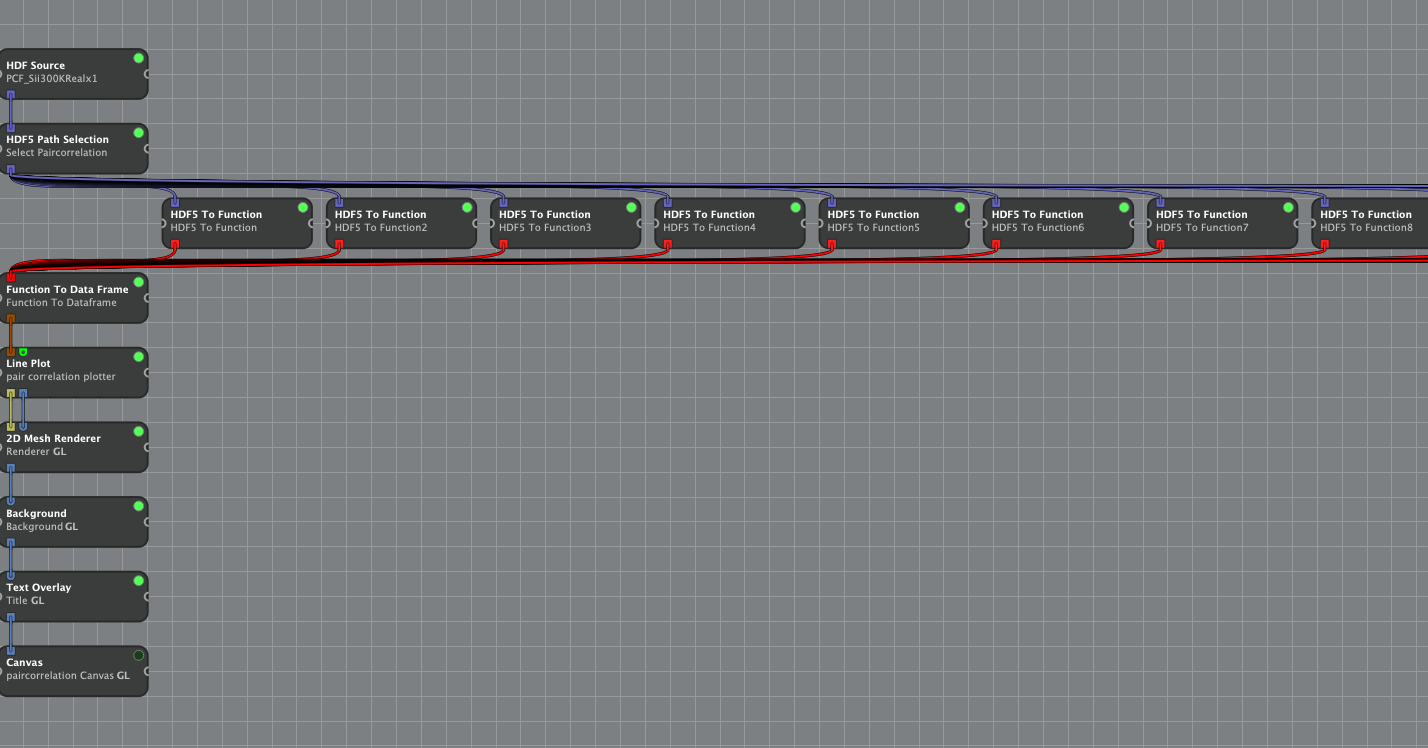
\includegraphics[width=1.00000\textwidth]{Images/PCF.png}
\caption{Nätverk för parkorrelationsfunktion.}
\label{fig:PCFnetwork}
\end{figure}

Nätverket startar med att öppna en HDF5-fil. Efter det kontrollerats om
gruppen \emph{PairCorrelationFunc} finns i den parsade filen med hjälp
av \emph{HDF5PathSelection}-processorn. Därefter läggs det till en
\emph{HDF5ToFunction}-processor som extraherar den parsade datan och gör
om det till en funktion. Nästkommande processorn, dvs \emph{LinePlot},
används för att rita upp den data som tas emot från föregående
processron. En mesh byggs upp med hjälp av
\emph{MeshRenderer}-processorn, \emph{Background}-processorn bygger upp
bakgrunden och \emph{TextOverlay}-processorn används för att skriva ut
text till canvasen. Figur \ref{fig:PCF} och \ref{fig:PCFnetwork} demonstrerar ett
exempel på ett nätverk och respektive 2D-graf som visualiserar
paircorrelation funktionen för Si med 40 steg i temperaturen 300K.
Observera att alla \emph{HDF5ToFunction}-processorer inte syns i figur
\ref{fig:PCF}. Den 2D-grafen som genereras av nätverken visas i figur
\ref{fig:PCF}.

\begin{figure}[H]
\centering
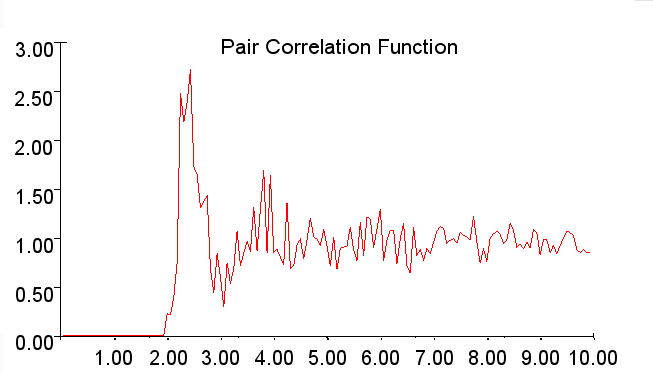
\includegraphics[width=1.00000\textwidth]{Images/network.png}
\caption{2D-graf från parkorrelationsfunktion.}
\label{fig:PCF}
\end{figure}

\subsubsection{Bandstruktur}\label{bandstruktur}

Nätverket startar med att öppna en HDF5-fil. Därefter skapas en process
som extraherar data. Sedan navigeras det genom HDF5-filen till platsen
där alla band, högkarakteristiska punkter (symboler) i Brillouin-zonen
och högkarakteristiska punkternas koordinater är sparade. Alla band
sparas i en DataFrame där varje kolumn innehåller alla värden för ett
band. Alla högkarakteristiska punkter med tillhörande koordinat sparas i
varsina DataFrames. Därefter ritas alla band och symboler upp. Det ritas
även upp linjer som ligger i lod med symbolerna för att enklare se var i
plotten symbolerna är. X-axeln visar symbolerna och y-axeln visar
energierna i eV. X-axeln är även baserad på antalet iterationer av
k-punkterna ur VASP-filerna.

Med den kunskapen gruppmedlemmarna besitter idag skulle inte x-axeln
vara baserad på iterationer av k-punkter utan på avståndet mellan två
symboler i Brillouin-zonen.

\begin{figure}[H]
\centering
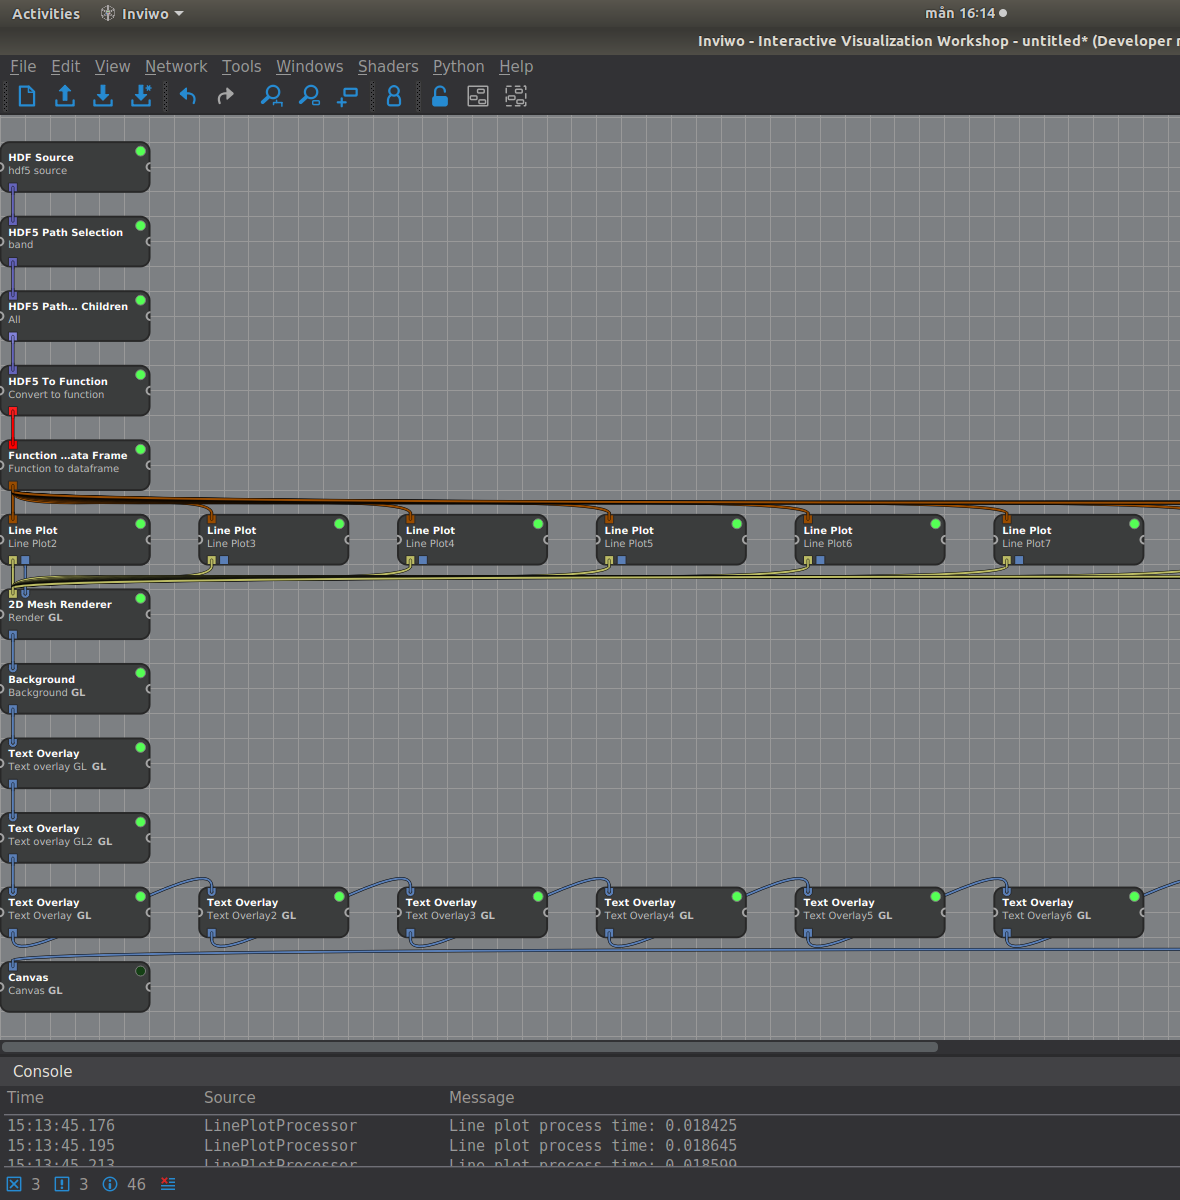
\includegraphics[width=0.9000\textwidth]{Images/network_bandstructure.png}
\caption{Nätverk för visualisering av bandstruktur.}
\end{figure}

\begin{figure}[H]
\centering
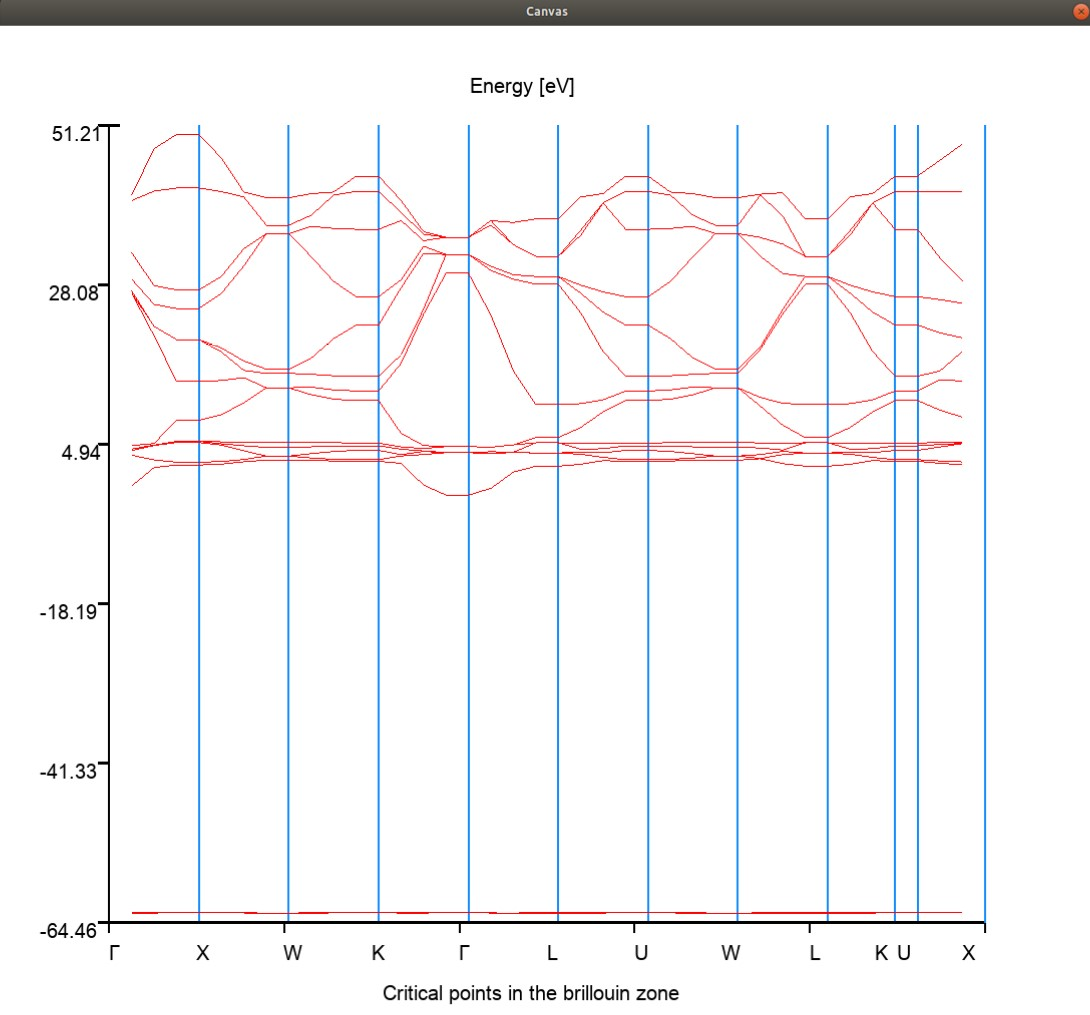
\includegraphics[width=0.90000\textwidth]{Images/new_bandstructure.jpg}
\caption{2D-graf för bandstruktur.}
\end{figure}

Plott över bandstrukturen med inmarkerade högkarakteristiska punkter
(symboler) och linjer för att markera symbolernas läge i plotten.

\subsubsection{Tillståndstäthet}\label{tillstuxe5ndstuxe4thet}

Nätverket för visualisering av tillståndstäthetsdata laddar en
\emph{HDFSource}-processor som anger HDF5-filen som data laddas från.
Sedan kopplas en \emph{HDF5PathSelection}-processor, som tar ut den
givna HDF5-gruppens alla undergrupper direkt till den redan befintliga
\emph{HDFSource}-processorn. Denna processor anger att data ska laddas
från DOS-gruppen i HDF5-filen. Två till
\emph{HDF5PathSelection}-processorer laddas sedan som anger grupperna
Total och Partial i HDF5-filen.

För Total-delen laddas sedan kontinuerligt
\emph{HDF5ToFunction}-processorer som gör funktioner av all data i
Total-gruppen. För Partial-gruppen laddas en
\emph{HDF5PathSelection}-processor som tar ut dataset för en vald atom
genom att välja den givna HDF5-filens relevanta undergrupp. Denna
processor har namnet \emph{Partial Pick} i nätverket. Därefter laddas
\emph{HDF5ToFunction}-processorer för alla dataset i grupperna under
Partial-gruppen. All data matas sedan in i en \emph{LinePlot}-processor
som gör en 2D-graf. Detta matas in i en \emph{Canvas}-processor som
visar själva grafen. Dessutom finns två textOverlay processorer som
skriver ut text för x- och y-axeln. Figur \ref{fig:DoS} visar total
tillståndstäthet för titanfosfat, TiPO4. Figur \ref{fig:DoSNetwork} visar
nätverket som ger 2D-grafen i figur \ref{fig:DoS}. Användaren kan även välja
att visa en 2D-graf av den partiella tillståndstätheten med hjälp av
sammma nätverk.

\begin{figure}[H]
\centering
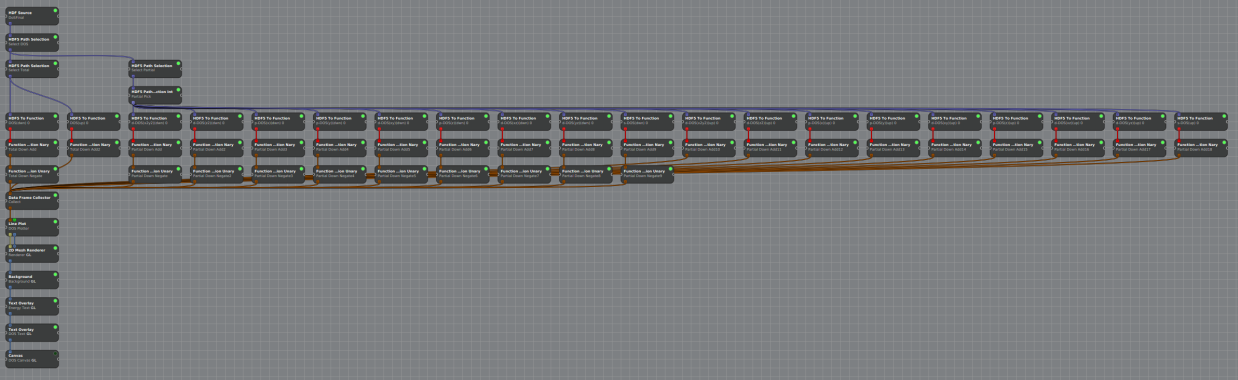
\includegraphics[width=1.00000\textwidth]{Images/DoSNetwork.PNG}
\caption{Nätverk för visualisering av tillståndstäthet.}
\label{fig:DoSNetwork}
\end{figure}

\begin{figure}[H]
\centering
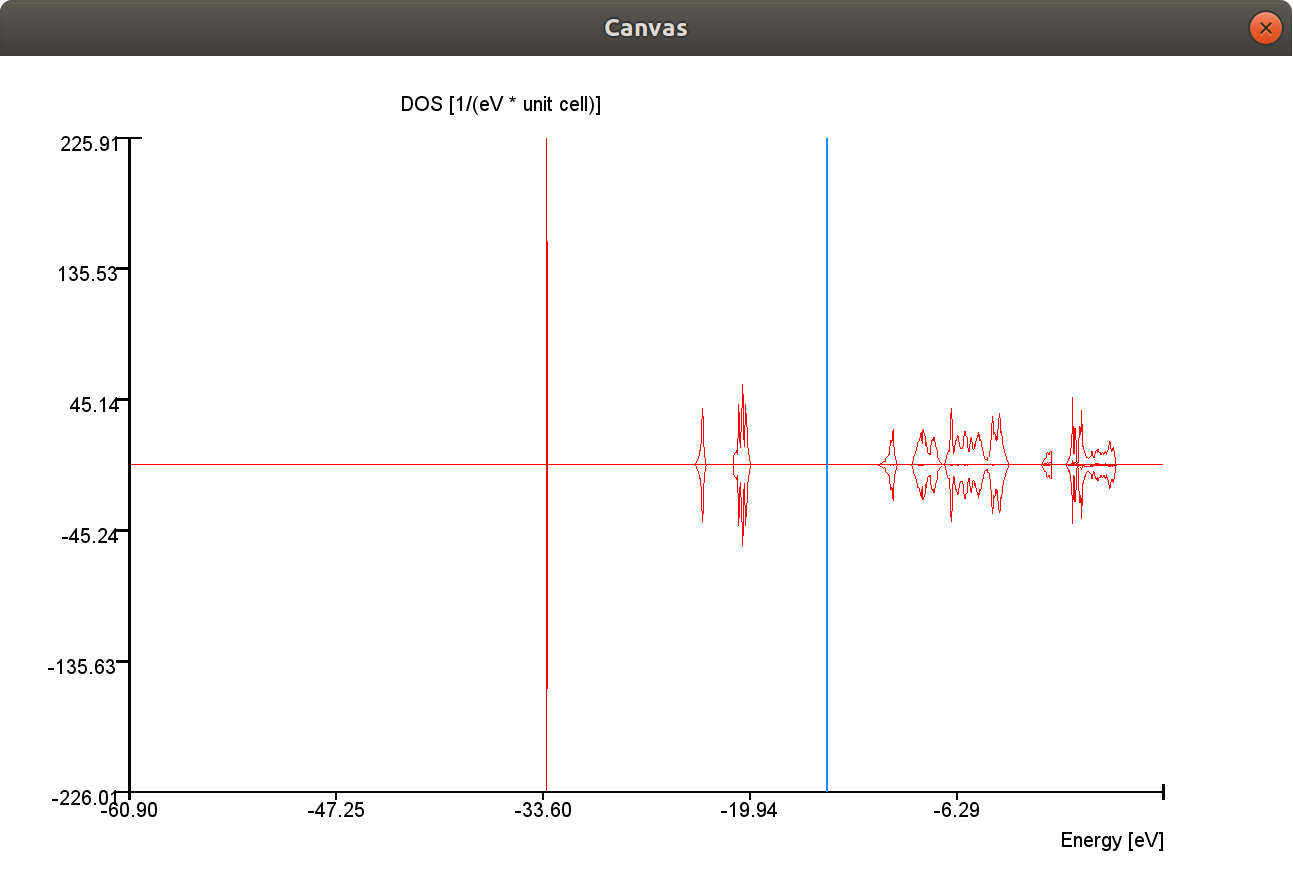
\includegraphics[width=1.0000\textwidth]{Images/TotalDoS.png}
\caption{Visualisering av tillståndstäthet för TiPO4.}
\label{fig:DoS}
\end{figure}

\begin{figure}[H]
\centering
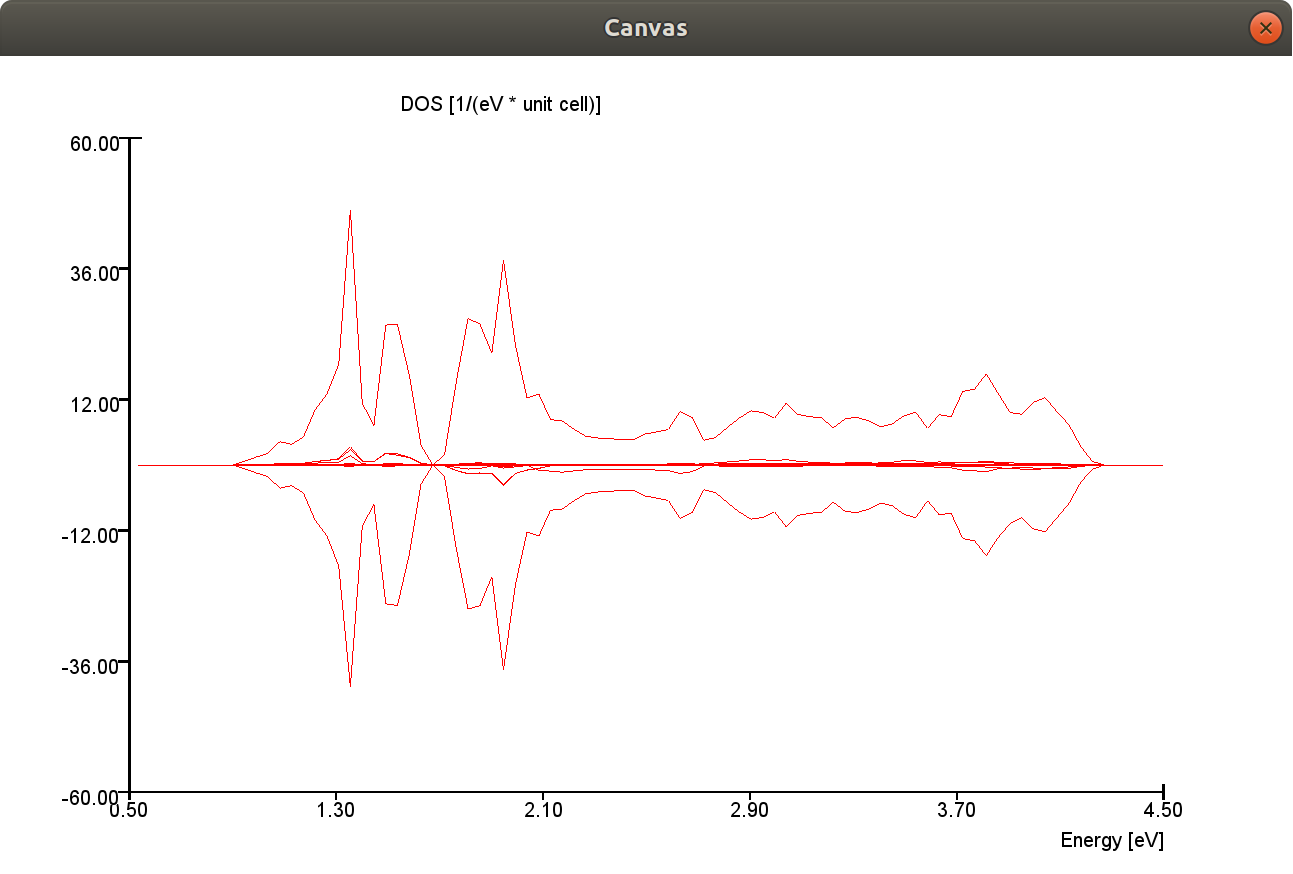
\includegraphics[width=1.0000\textwidth]{Images/ZoomedDoS.png}
\caption{Inzoomad visualisering av tillståndstäthet för TiPO4.}
\end{figure}



\subsubsection{Enhetscell}\label{enhetscell}

Hos nätverket för visualisering av enhetscellen hämtar först en
\emph{HDFSource}-processor HDF5-filen. Under \emph{HDFSource}-processorn
ligger ett antal \emph{CoordinateReader}-processorer, en för varje
atomslag i enhetscellen. Från HDF5-filen hämtar var och en av
\emph{CoordinateReader}-processorerna koordinaterna för atomslagens alla
enhetscellsatomer. En \emph{StructureMesh}-processor skapar sedan en
mesh utifrån koordinaterna. Efter det skapar en
\emph{SphereRenderer}-processor en bild utifrån meshen, där en sfär
ritas ut för varje atom i enhetscellen. Bilden skickas sedan till en
\emph{Canvas}-processor, som skapar ett fönster där bilden visas.
Figuren nedan visar hur nätverket ser ut för bariumsulfat (BaSO4) och
figuren under den visar den resulterande bilden.

\begin{figure}[H]
\centering
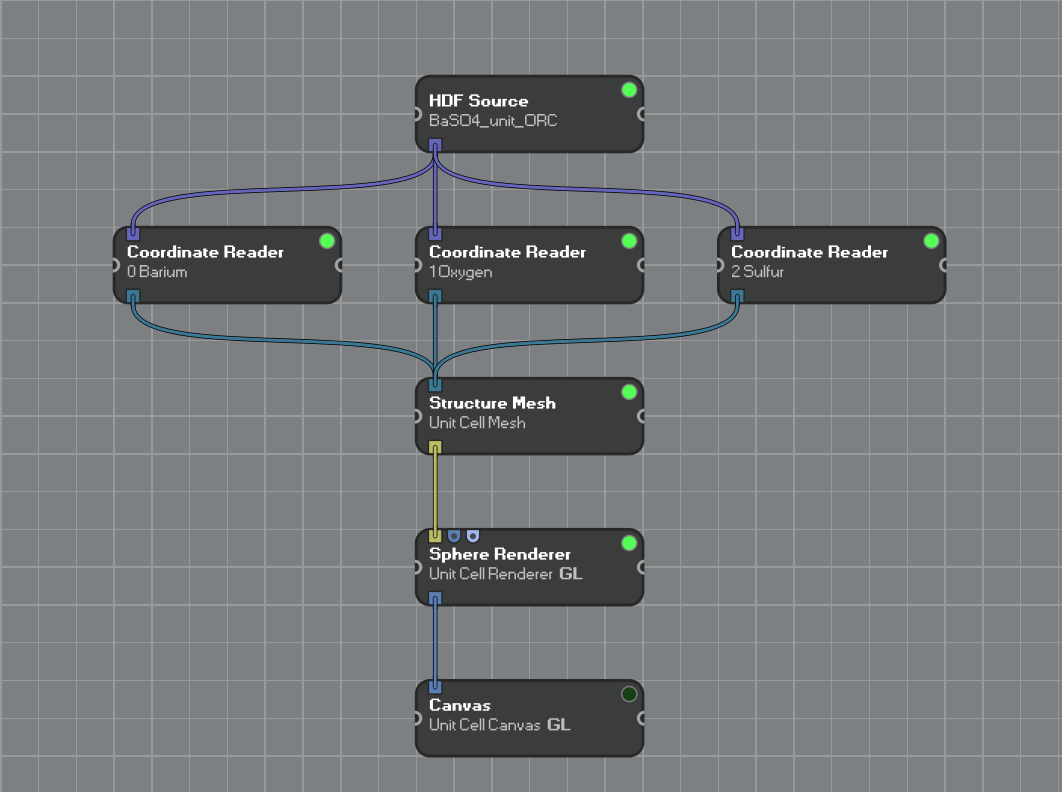
\includegraphics[width=0.60000\textwidth]{Images/unitcell_network.png}
\caption{Nätverk för visualisering av enhetscellen.}
\end{figure}

\begin{figure}[H]
\centering
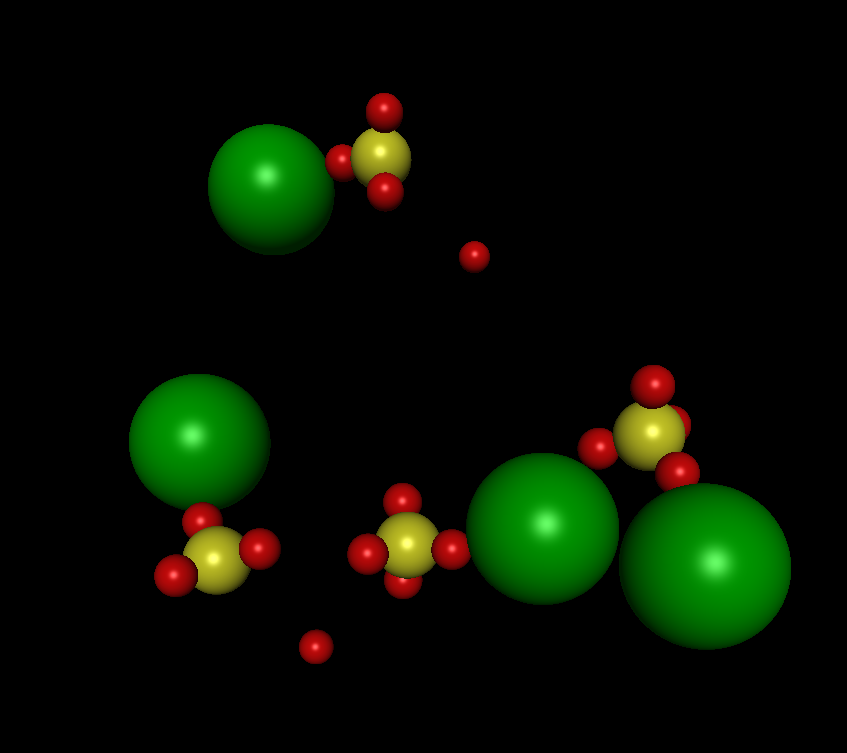
\includegraphics[width=0.60000\textwidth]{Images/unitcell.png}
\caption{Den resulterande bilden.}
\end{figure}

\subsubsection{Fermi-yta}\label{fermi-yta}

Visualisering av fermi ytan görs med en skapad python process
\emph{HDF5FermiSource}. \emph{HDF5FermiSource} läser in en hdf5 fil
skapad av parsesystemen. Genom attributet \emph{energy\_band} väljs
vilken data ska visualiseras, datan normalisersas och sedan omvandlas
till en \emph{Inviwo-Volume} som output. Resterande delarana av
nätverket är inbygga inviwo processorer. Volymen skickas till två mesh
renderare som omvandlare meshen till en bild. \emph{ISO-Raycaster} kan
sedan välja ut vilka värden i volymen att visa i den resulterande bilden
som \emph{Canvas} målar upp.

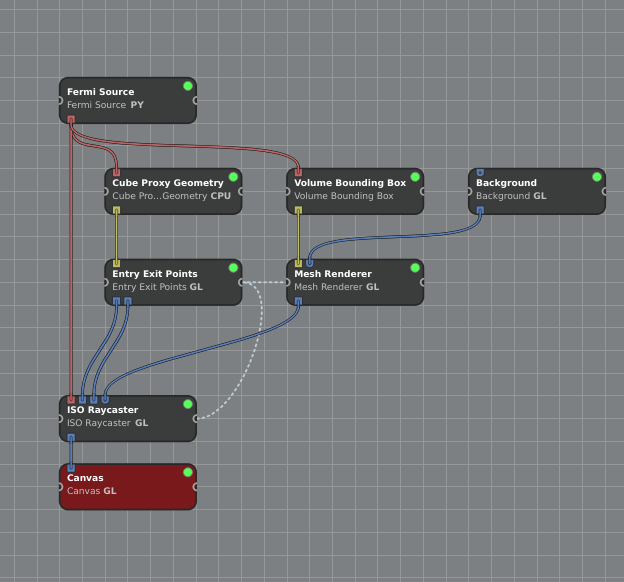
\includegraphics[width=0.49000\textwidth]{Images/fermi_network.png}

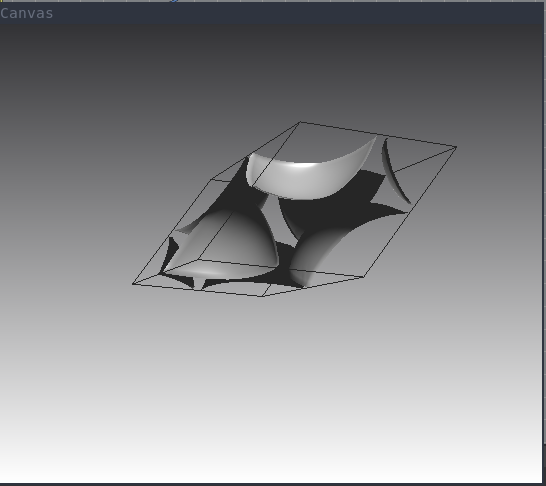
\includegraphics[width=0.49000\textwidth]{Images/fermi_canvas.png}

\emph{Fermi-yta (höger) Inviwo-nätverket (vänster) resulterande bild.}

\subsubsection{Elektrontäthet}\label{elektrontuxe4thet}

Figuren nedan visar nätverket för visualisering av elektrontäthet. Först
hämtar en \emph{HDFSource}-processor HDF5-filen. En
\emph{HDF5ToVolume}-processor hämtar sedan elektrontätheten från
HDF5-filen och genererar en volym för den. Processorerna
\emph{CubeProxyGeometry}, \emph{EntryExitPoints} och
\emph{VolumeRayCasyer} skapar en bild utifrån volymen. Denna bild är en
3D-bild av elektrontätheten hos materialets enhetscell. Processorerna
\emph{VolumeBoundingBox} och \emph{MeshRenderer} skapar en
parallellepiped som omsluter volymen. Parallellepipeden skickas sedan
vidare till \emph{VolumeRayCaster}-processorn, där den sammanfogas med
elektrontäthetsbilden. Till den resulterande bilden läggs det sedan på
en bakgrund med hjälp av en \emph{Background}-processor. Slutligen
skickas bilden till en \emph{Canvas}-processor, som gör att bilden visas
upp.

Volymen som skapas av \emph{HDF5ToVolume}-processor skickas även
parallellt till en \emph{VolumeSlice}-procssor, som genererar ett
tvådimensionellt tvärsnitt av elektrontätheten. Till den läggs det sedan
till en bakgrund med hjälp av en \emph{Background}-processor och
slutligen skickas tvärsnittsbilden till en egen \emph{Canvas}-processor,
där den visas upp.

\begin{figure}[H]
\centering
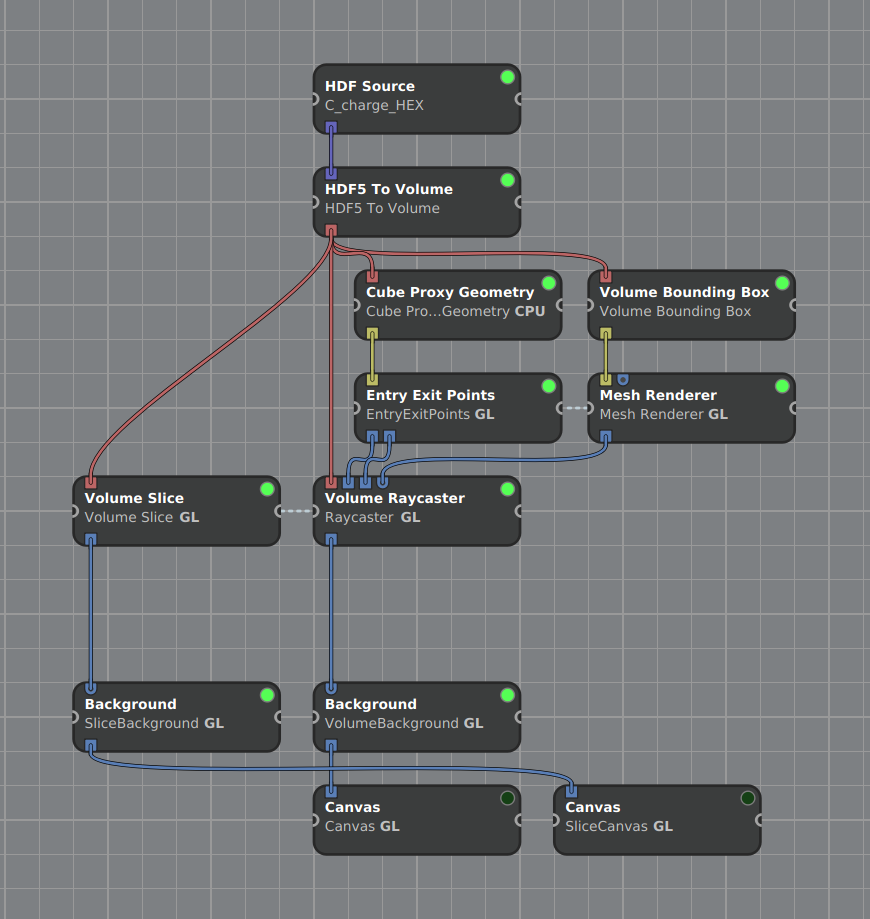
\includegraphics[width=0.60000\textwidth]{Images/charge_network.png}
\caption{Nätverket för visualisering av elektrontäthet.}
\end{figure}

\begin{figure}[H]
\centering
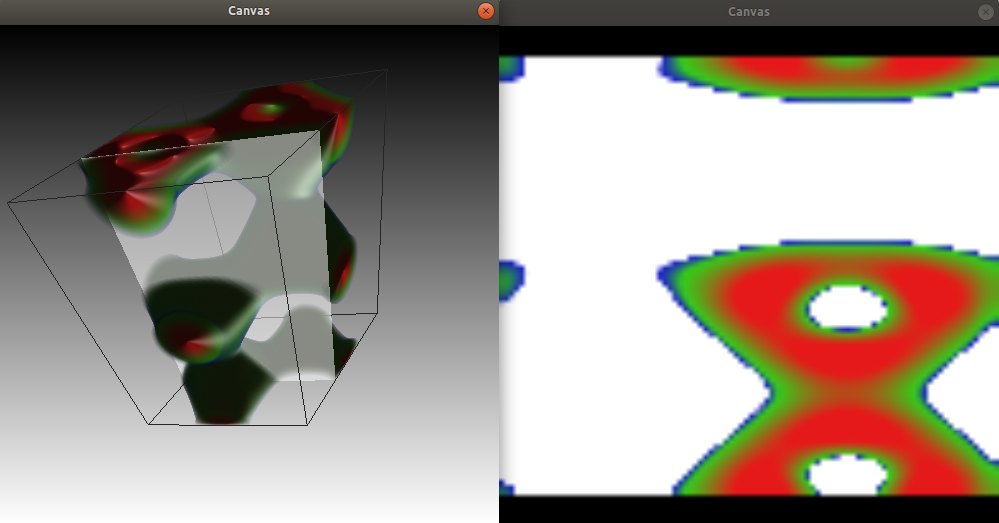
\includegraphics[width=0.60000\textwidth]{Images/charge.png}
\caption{De resulterande bilderna.}
\end{figure}

\subsubsection{Molekyldynamik}\label{Molekyldynamik}
Nätverket för visualisering av molekyldynamik hämtar först en HDF5-fil med hjälp av en \emph{HDFSource}-processor. För varje typ av atom finns en \emph{CoordinateReader}-processor som hämtar data från HDF5-filen. Denna data består av information om atomernas position i ett tidssteg. Varje \emph{CoordinateReader}-processor är kopplad med en \emph{Property Animator}-processor. En \emph{Property Animator}-processor kan ändra olika egenskaper hos \emph{CoordinateReader}-processorn. Exempel på dessa är vilken typ av animering som ska ske, hur snabbt resultatet ska animeras och om det ska finnas en fördröjning i resultatet. \emph{StructureMesh}-processorn skapar sedan ett mesh utifrån atomernas koordinater. Sedan ritar en \emph{SphereRender}-processor ut en bild av atomerna, representerade som sfärer. Till den resulterande bilden läggs sedan en bakgrund, med hjälp av en \emph{Background}-processor. Sedan ritas det grafiska resultatet ut av en \emph{Canvas}-processor.

\begin{figure}[H]
\centering
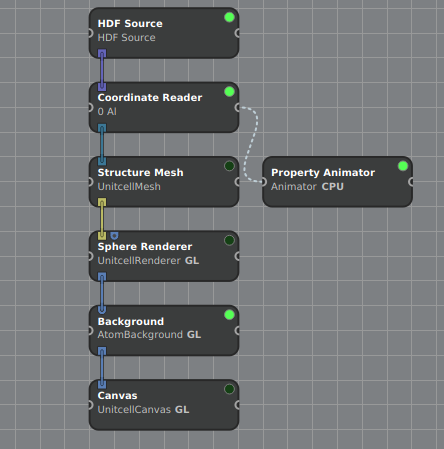
\includegraphics[width=0.60000\textwidth]{Images/moldyn_network.png}
\caption{Nätverket för visualisering av molekyldynamik.}
\end{figure}

\begin{figure}[H]
\centering
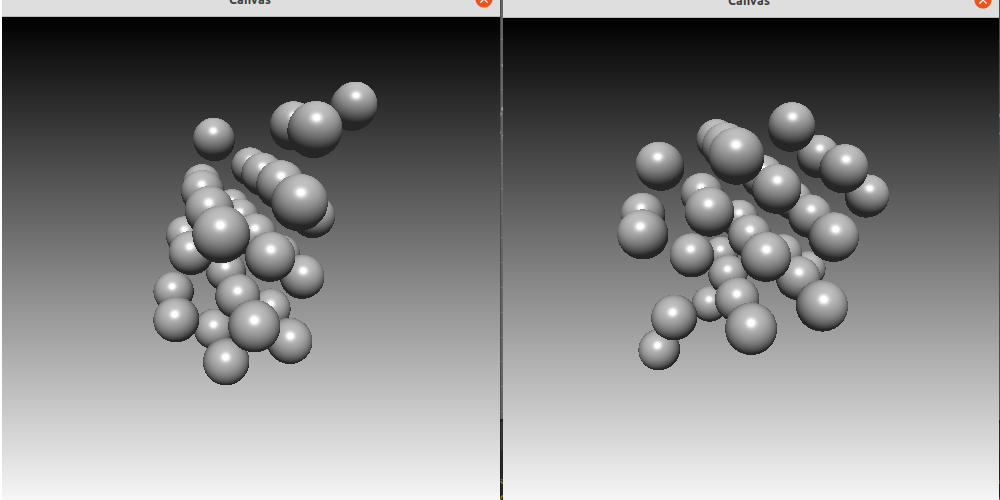
\includegraphics[width=0.60000\textwidth]{Images/moldyn_visualisering.png}
\caption{Grafiskt resultat av molekyldynamiksvisualiseringen. Bilden visar atomernas positioner vid två olika tidpunkter.}
\end{figure}

\subsubsection{Kraftvektorer}\label{Kraftvektorer}
I nätverket för kraftvektorer hämtas HDF5-filen med hjälp av en \textit{HDF Source} processor. Denna är sedan inkopplad i lika många \textit{Coordinate Reader} processorer som det finns typer av atomer i HDF5-filen. En \textit{Structure Mesh} processor följt av en \textit{Sphere Renderer} processor skapar atomerna och dess attribut i 3D.

Vektorerna alstras från \textit{Composite} processorn till höger, den består av en samling \textit{Mesh Creator} processorer, en för varje vektor. En \textit{Mesh Renderer} processor skapar sedan vektorerna och dess attribut i 3D.

Slutligen skickas all atom och vektorinformation igenom en \textit{Background} processor och \textit{Canvas} processor där visualiseringen åskådliggörs.

\begin{figure}[H]
\centering
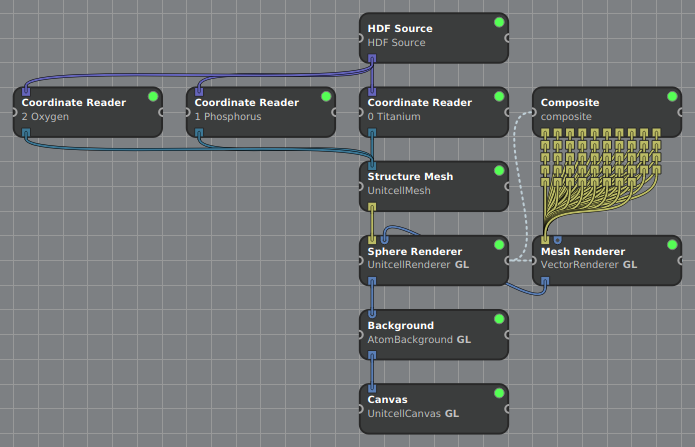
\includegraphics[width=1.00000\textwidth]{Images/force_network.png}
\caption{Nätverket för visualiseringar av kraftvektorer.}
\end{figure}

\begin{figure}[H]
\centering
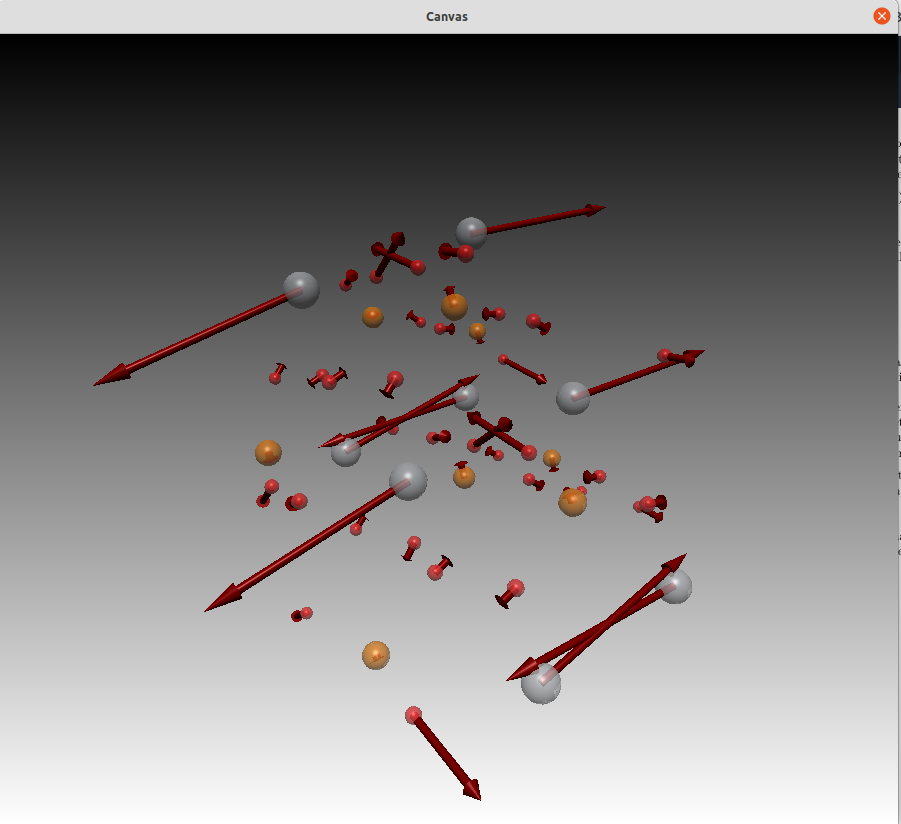
\includegraphics[width=0.60000\textwidth]{Images/force_vectors.png}
\caption{Visualisering av kraftvektorer.}
\end{figure}

\begin{figure}[H]
\centering
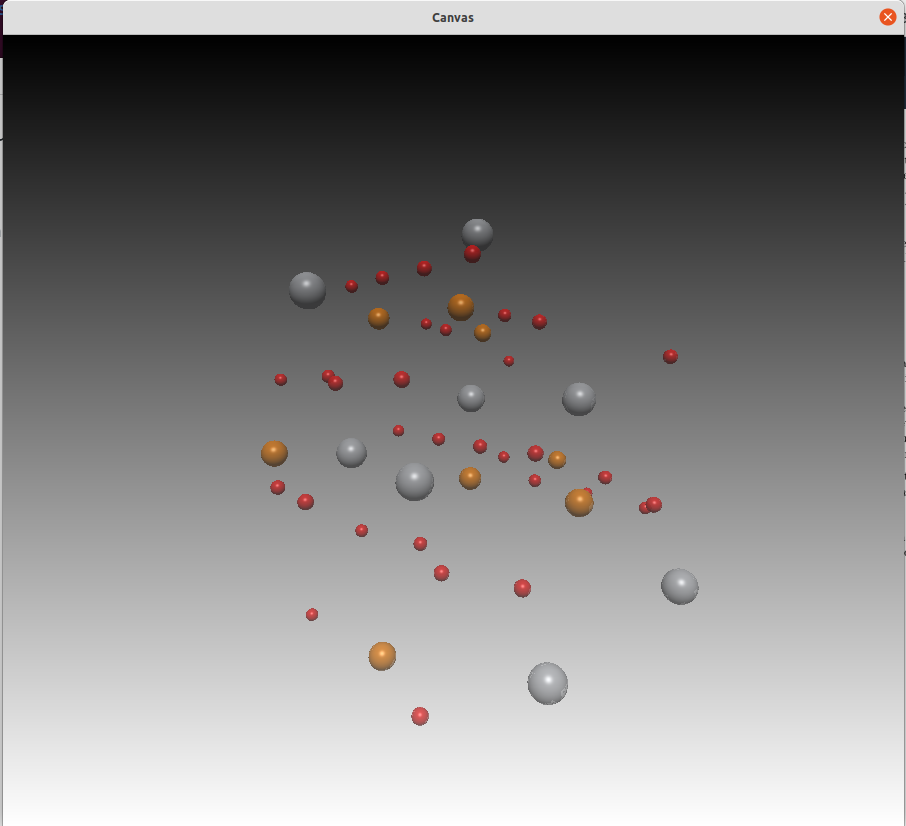
\includegraphics[width=0.60000\textwidth]{Images/force_vectors_disabled.png}
\caption{Visualisering av samma struktur utan kraftvektorer.}
\end{figure}


\subsection{NetworkManager och
Subnetwork}\label{networkmanager-och-subnetwork}

För att hantera mer avancerade inviwonätverk och för att kunna köra
flera visualiseringar parallellt så finns en pythonklass
\emph{Subnetwork}. Implementationer av denna klass har i uppgift att
överse en specifik visualisering och har funktioner för att sätta upp
och påverka denna visulisering. Alla visualiseringar som ska startas via
detta system kräver att en klass vilken ärver \emph{Subnetwork} skapas.
Se filen \emph{ExampleSubnetwork.py} för ett exempel på hur en klass som
ärver \emph{Subnetwork} bör implementeras.

En klass för att hantera de \emph{Subnetworks} som intieras har också
skapats. Denna heter \emph{NetworkManager}.
\emph{NetworkManager}-klassen har funktioner för att initera och spara
olika \emph{Subnetworks}. Den hanterar också interaktion mellan olika
\emph{Subnetworks} då detta behövs.

Filer relaterade till detta ligger under \emph{envisionpy}-modulen i
\emph{envisionpy/network}.

För nuvarande så finns de visualiseringar relaterade till
2d-grafvisualisering inte implementerade i detta system. Dessa använder
fortfarande det gamla \emph{NetworkHandler}-systemet.

\subsection{NetworkHandlers}\label{networkhandlers}

Detta system är ersatt med \emph{NetworkManager och Subnetwork} som beskrivs i ovanstrående kapitlet. Kapitlet finns kvar då det
beskriver hur visualiserningarna fungerar även om det inte längre är det
som används för att implementera nya visualiserningar.

För att andra delsystem enkelt ska kunna sätta upp och ändra parametrar
i inviwonätverken så har python-klasser, kallade \emph{NetworkHandlers},
skrivits. Dessa klasser initierar specifika delar av nätverket och har
funktioner för att ändra speciella properties i de processorer de har
ansvar över. \emph{NetworkHandlers} finns för nuvarande inte för alla
visualiseringar utan bara för de relaterade till volymrendering.

Alla dessa klasser ärver en basklass kallad \emph{NetworkHandler}. Denna
har i uppgift att ta hand om ett set av processorer som hör till en
speciell visualisering.

NetworkHandler-klasserna tillhör envisionpy-modulen och ligger under
envisionpy.processor\_network.

\subsubsection{VolumeNetworkHandler}\label{volumenetworkhandler}

En klass som sätter upp ett generiskt nätverk för volymrendering.
Nätverket som byggs upp kan inte självstående ge upphåv till någon
visualisering då ingen volymdatakälla initieras. Detta måste istället
göras från en mer specificerad \emph{VolumeHandler}-klass som ärver
denna.

\begin{figure}[H]
\centering
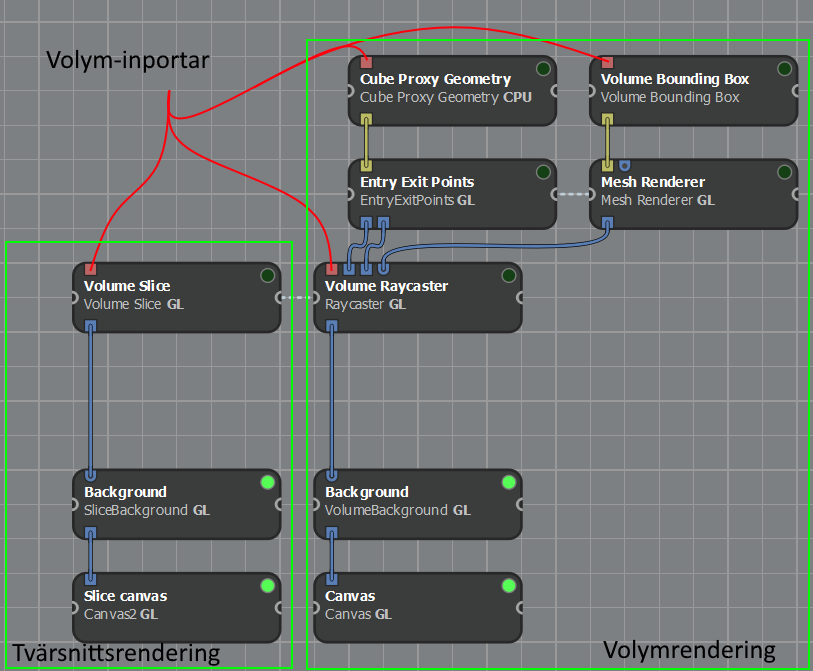
\includegraphics[width=1.00000\textwidth]{Images/volume_network_ex.PNG}
\caption{Nätverket som byggs upp då en VolumeNetworkHandler-instans
initieras.}
\label{fig:VolumeNetworkHandler}
\end{figure}

Som visas i figur \ref{fig:VolumeNetworkHandler} så kan nätverket delas upp
i två delar. En volymrenderingsdel och en tvärsnittsrenderingsdel.

Processorerna \emph{Cube Proxy Geometry}, \emph{Entry Exit Points}, och
\emph{Volume Raycaster}, visade i mitten av figur
\ref{fig:VolumeNetworkHandler} kommer att generera bilddata direkt baserat
på den volymdata de tar emot.

Processorerna \emph{Volume Bounding Box} och \emph{Mesh Renderer} visade
i högra delen av figur \ref{fig:VolumeNetworkHandler} kommer att generera
bilddata av den parallellepiped som stänger in volymen. Bilddatan
skickas sedan till \emph{Volume Raycaster} och sammanfogas där med
bilddatan av volymen. Detta skickas sedan till \emph{Volume
Background}-processorn där en bakgrund adderas till bilddatan som sedan
skickas till \emph{Canvas}-processorn där den slutgiltiga
visualiseringen visas.

Tvärsnittsrenderingen tar emot samma volymdata som volymrenderingen,
skickar det till \emph{Volume Slice}-processorn, vilken genererar
bilddata baserat på ett plan som skär volymen. Bilddatan skickas sedan
till en egen canvas. Volymrenderingens \emph{Raycaster}-processor har
förmågan att rita ut ett plan på en godtycklig position i volymen. Detta
plan länkas till planet i \emph{Volume Slice}-processorn så att ett
delvis transparent plan ritas i volymen på samma position som planet
\emph{Volume Slice} använder sig av för att hämta sin data.
Tvärsnittsrenderingen kan aktiveras och inaktiveras genom att dess
\emph{Canvas}-processor raderas eller läggs till, och att
planrenderingen i \emph{Raycaster}-processorn aktiveras eller
inaktiveras.

\subsubsection{UnitcellNetworkHandler}\label{unitcellnetworkhandler}

En klass som sätter upp ett och hanterar nätverk för
atompositionsrendering. Nätverket som sätts upp kan självstående
generera en visualisering för bara atompotitioner men kan också
kombineras med andra nätverk genom att denna ärvs i mer specificerade
\emph{NetworkHandler}-klasser.

\begin{figure}[H]
\centering
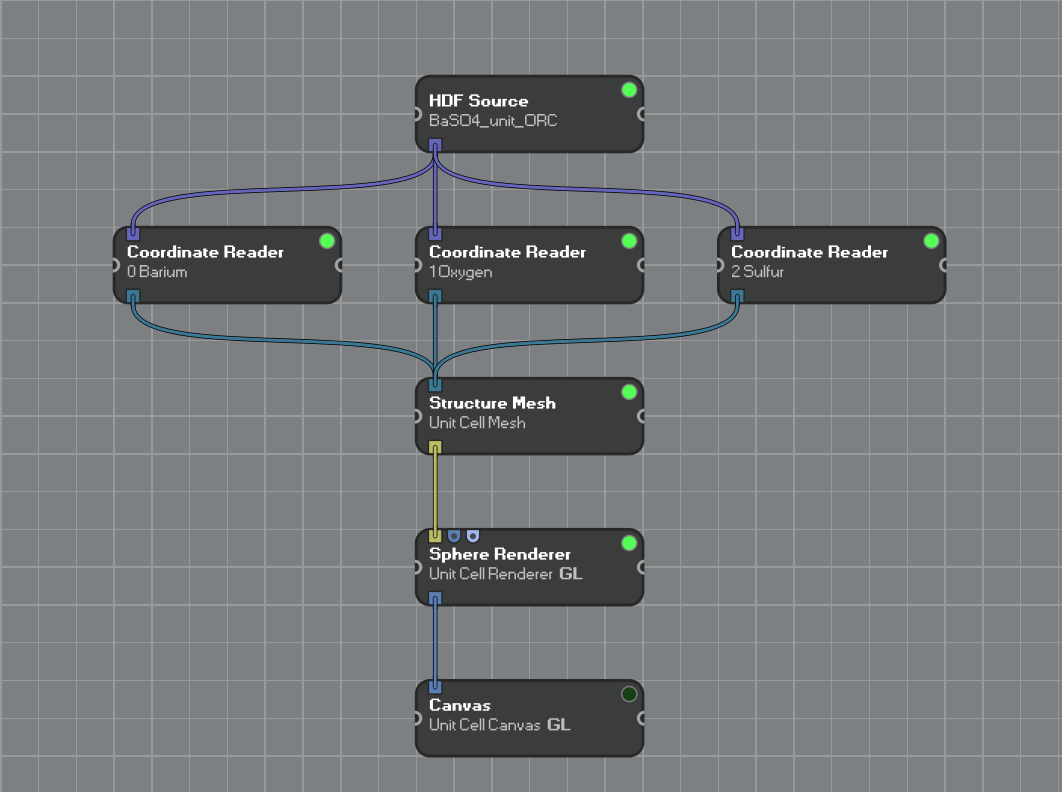
\includegraphics[width=0.60000\textwidth]{Images/unitcell_network.png}
\caption{Nätverket som byggs upp då en UnitcellNetworkHandler-instans
initieras.}
\label{fig:UnitcellNetowrkHandler}
\end{figure}

\begin{figure}[H]
\centering
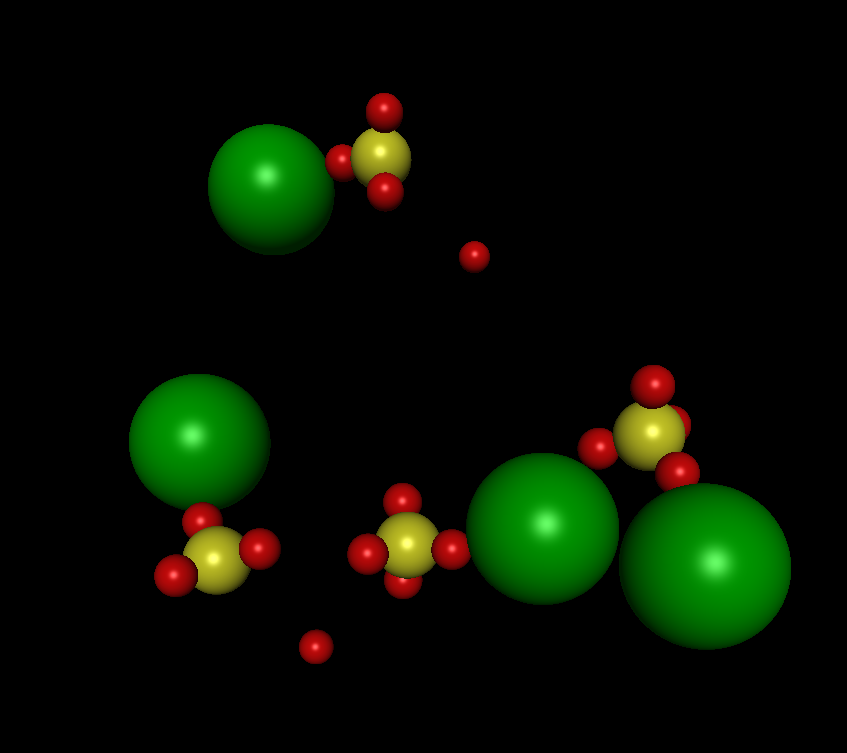
\includegraphics[width=0.60000\textwidth]{Images/unitcell.png}
\caption{Resulterande bild från nätverk i figur
\ref{fig:UnitcellNetowrkHandler}}
\end{figure}

\emph{UnitcellNetworkHandler} börjar med kontrollera att den givna
HDF5-filen har data för en atompositionsvisualisering och kastar ett
\emph{AssertionError} om den inte har det. Den fortsätter sedan med att
sätta upp en \emph{HDF5 Source}-processor, om en sådan redan existerar
så används den existerande processorn istället. Vilka atomtyper som
HDF5-filen innehåller information om läses sedan.

En \emph{Coordinate Reader}-processor för varje atomtyp läggs till.
Koordinatdatan skickas vidare till en \emph{Structure Mesh}-processor,
en ENVISIoN processor som konverterar koordinaterna till en \emph{mesh}.
Meshen skickas till \emph{Sphere Renderer} där den konverteras till
bilddata med en sfär vid varje tidigare koordinat. Bilddatan ritas sedan
ut på en \emph{Canvas}.

\subsubsection{ChargeNetworkHandler}\label{chargenetworkhandler}

En specificerad klass för att sätta upp och hantera
laddningstäthetsvisualiseringen. Klassen genererar ett fullständigt
nätverk för laddningstäthetsvisualisering och har funktioner för att
alla parameterändringar som där behövs. Ärver
\emph{VolumeNetworkHandler} för att hantera volymrenderingsaspekten av
visualiseringen.

\begin{figure}[H]
\centering
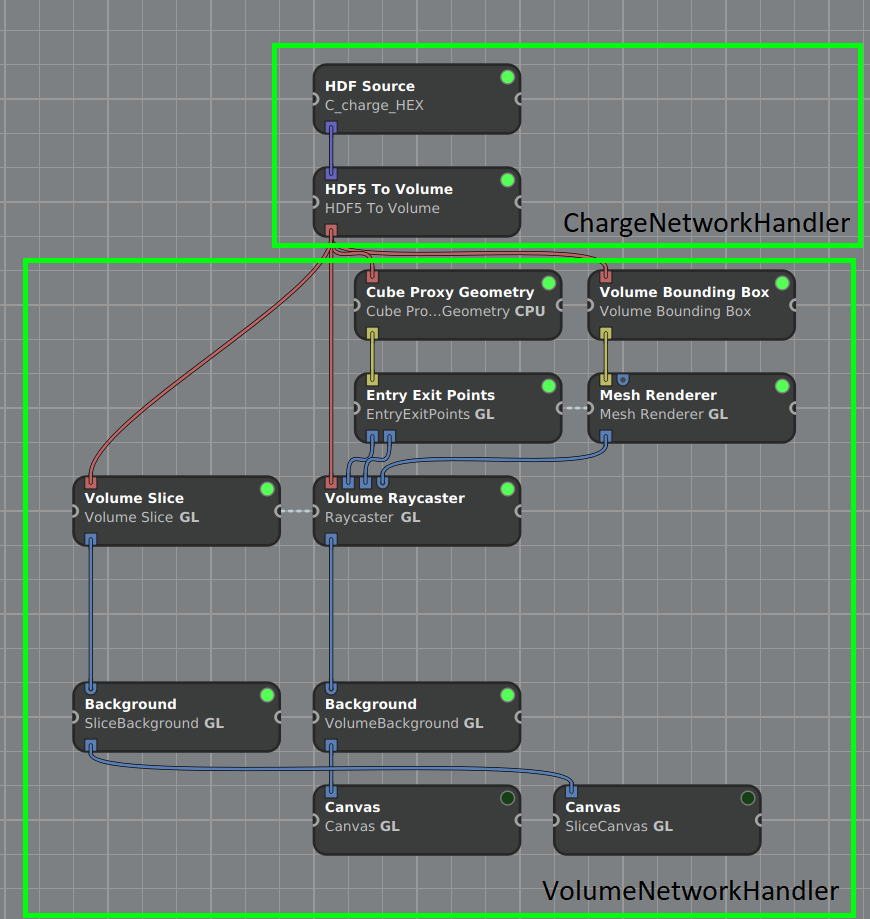
\includegraphics[width=0.60000\textwidth]{Images/ChargeNetworkHandler.png}
\caption{Nätverket som byggs upp då en ChargeNetworkHandler-instans
initieras.}
\label{fig:ChargeNetworkHandler}
\end{figure}

\begin{figure}[H]
\centering
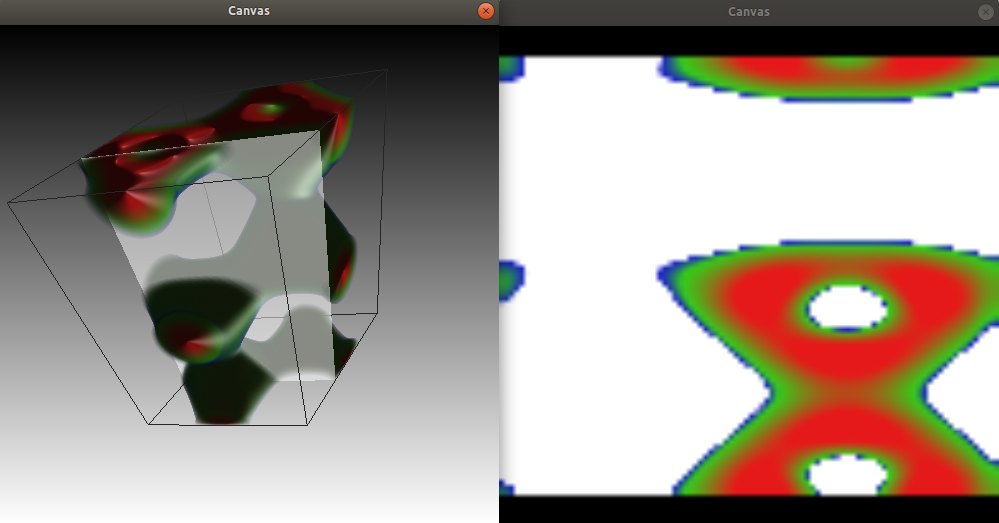
\includegraphics[width=0.60000\textwidth]{Images/charge.png}
\caption{Resulterande bild från nätverk i figur \ref{fig:ChargeNetworkHandler}}
\end{figure}

\emph{ChargeNetworkHandler} börjar med kontrollera att den givna
HDF5-filen har data för en laddningstäthetsvisualisering och kastar ett
\emph{AssertionError} om den inte har det. Den fortsätter sedan med att
initera sin superklass \emph{VolumeNetworkHandler}. Denna sätter up sin
del av nätverket som indikerat i figur \ref{fig:ChargeNetworkHandler}.

En \emph{HDF5 Source} sätts upp och sedan sätts en \emph{HDF5 To Volume}
upp och anslutes till \emph{HDF5 Source}. \emph{HDF5 To Volume} hämtar
ut volymdata från HDF5-filens \emph{/CHG/} sökväg. Processorn genererar
volymdata som i sin tur ansluts med volymrenderingsdelens
volymdatainportar.

\subsubsection{ELFNetworkHandler}\label{elfnetworkhandler}

ELFNetworkHandler är identisk i jämförelse med ChargeNetworkHandler med
ett fåtal skillnader. Volymdata från HDF5-filen hämtas från sökvägen
\emph{/ELF/} istället för \emph{/CHG/}. Detta gör att funktioner för att
hämta och sätta aktiva band också är olika.

\subsubsection{ParchgNetworkHandler}\label{parchgnetworkhandler}

En specificerad klass för att sätta upp och hantera visualiseringen för
partiell laddningstäthet. Ärver \emph{VolumeNetworkHandler} och
\emph{UnitcellNetworkHandler} för att hantera volymrenderingsaspekten
respektive atompositionsaspekten av visualiseringen.

\begin{figure}[H]
\centering
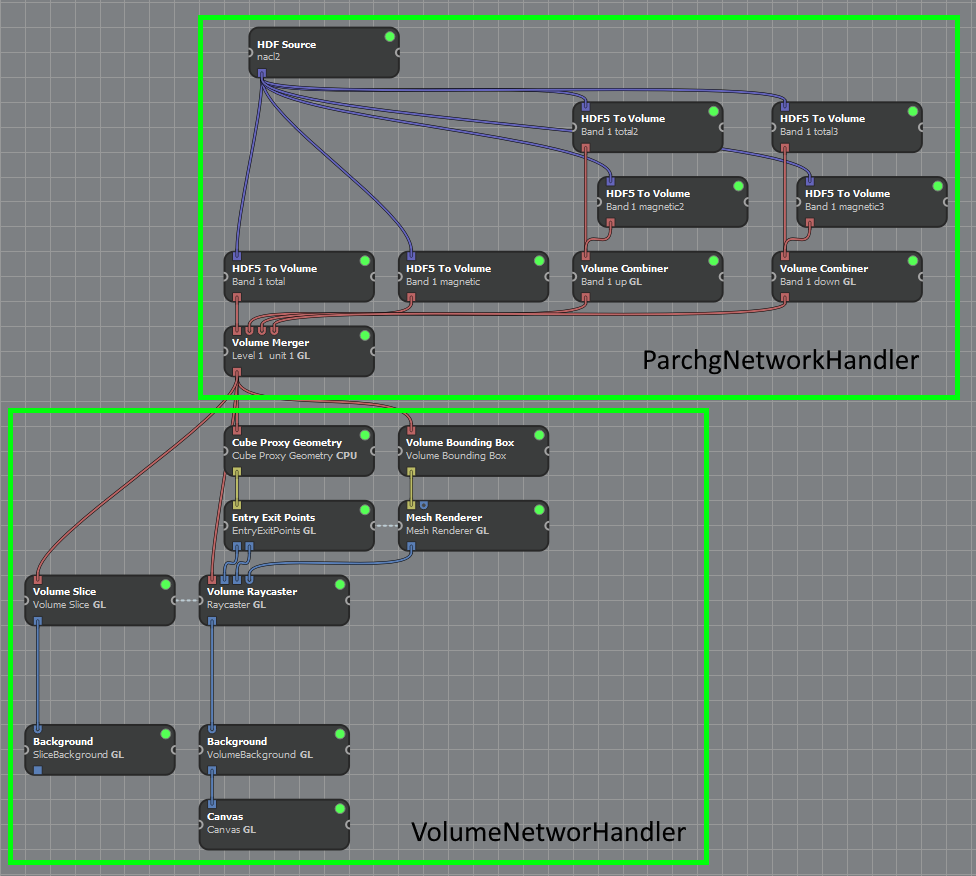
\includegraphics[width=1.00000\textwidth]{Images/parchg_network_ex.png}
\caption{Nätverket som byggs av ParchgNetworkHandler (utan
atompositionsrendering).}
\end{figure}

Till att börja med initieras superklassen \emph{VolumeNetworkHandler}
detta sätter upp det generiska volymrenderingsnätverket.

Efter detta initieras volymdatakällan och volymdataoutporten ansluts
till volymrenderingsdelen av nätverket.

Volymkällan är här mer komplicerad i jämförelse mot övriga
visualiseringar, eftersom flera olika volymdataset här ska visualiseras
som en volym. Precis hur denna del ser ut beror på de bandval som görs
av användaren.

\begin{figure}[H]
\centering
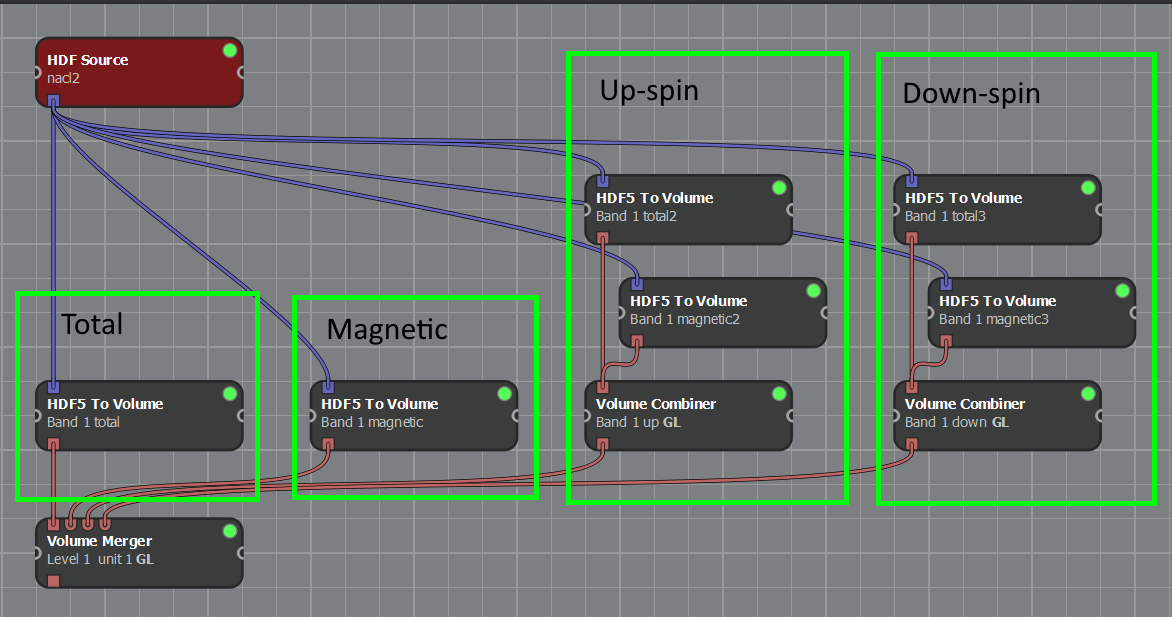
\includegraphics[width=1.00000\textwidth]{Images/parchg_source_ex.png}
\caption{Exempel på nätverkets volymdatakälla med ett bandval för varje
läge.}
\end{figure}

Den partiella laddningstäthetsvisualiseringen tillåter användaren att
välja ett godtyckligt antal band som ska visualiseras och ett av fyra
olika lägen för varje band. Dessa lägen är \emph{Total},
\emph{Magnetic}, \emph{Up-spin}, och \emph{Down-spin}. De olika lägena
hämtar ut volymdata ur HDF5-filen på olika sätt.

\begin{itemize}
\tightlist
\item
  \textbf{Total:} Hämtar direkt volymdatan från det valda bandets
  \emph{/total/} sökväg.
\item
  \textbf{Magnetic:} Hämtar direkt volymdatan från det valda bandets
  \emph{/magnetic/} sökväg.
\item
  \textbf{Up-spin:} Hämtar ut både \emph{/total/} och \emph{/magnetic/}
  volymdatan som \emph{v1} och \emph{v2}. Volymerna summeras sedan med
  formeln \emph{0.5}*(v1+v2)
\item
  \textbf{Down-spin:} Hämtar ut både \emph{/total/} och
  \emph{/magnetic/} volymdatan som \emph{v1} och \emph{v2}. Volymerna
  summeras sedan med formeln \emph{0.5}*(v1-v2)
\end{itemize}

Volymdatan från de olika bandvalen kombineras sedan med en \emph{Volume
Merger}-processor. \emph{Volume Merger} kan summerar upp till fyra
volymer till en. Om mer än fyra bandval har gjorts så används flera
lager av \emph{Volume Merger}-processorer för att kunna summera alla
dessa till en. Volymdatan från den sista \emph{Volume Merger} skickas
sedan till volymrenderingsnätverket.

\subsubsection{LinePlotNetworkHandler}\label{lineplotnetworkhandler}

Hanterar den generella delen av en 2D-graf visualisering. Styr allt som
har med 2D-grafen att göras, som skalning, axlar på grafen, med mera.

\subsubsection{BandstructureNetworkHandler}\label{bandstructurenetworkhandler}

Ärver LinePlotNetworkHandler och sätter upp den specifika delen för
bandstructure visualiseringen. Styr HDF5-källan och bandval.

\subsubsection{DOSNetworkHandler}\label{dosnetworkhandler}

Ärver LinePlotNetworkHandler och UnitcellNetworkHandler och sätter upp
den specifika delen för tillståndstäthets visualiseringen. Styr
HDF5-källan och val av tillstånd.

\subsubsection{PCFNetworkHandler}\label{pcfnetworkhandler}

Ärver LinePlotNetworkHandler och sätter upp den specifika delen för
parkorrelationsfunktions visualiseringen. Styr HDF5-källan och val av
tidssteg.

\subsubsection{FermiSurfaceNetworkHandler}\label{fermisurfacenetworkhandler}

Ärver Network handler och skapar en gränsnitt med några
\emph{Inviwo-properties}. Specifict i \emph{HDF5FermiSource}:
\emph{energy\_band} \emph{expand}, \emph{brillouin\_zone} och
\emph{ISO-Raycaster}: \emph{iso-value}. Mer detaljer finns i respective
\emph{Inviwo-process} dokumentation.

\subsection{Datastrukturer}\label{datastrukturer}

Två datastrukturer, Point och Function, har introducerats. En
datastruktur är en form av behållare av olika typer av data som kan
skickas mellan processorer. Dessa används i vissa av de implementerade
processorerna.

\subsubsection{Point}\label{point}

Denna datatyp representerar en reell 1D-punkt och inkapslar punktens
värde (ett flyttal) samt variabel metadata.

\subsubsection{Function}\label{function}

Denna datatyp representerar en reellvärd funktion av en reell variabel
och inkapslar sampelvärden och variabel-metadata för x- och y-axlarna.

\subsection{Processorer}\label{processorer}

För att kunna omvandla den data som översatts från VASP-beräkningar till
en visualisering krävs processorer som utför specifika uppgifter. Figur
\ref{fig:Processor} demonstrerar ett typiskt utseende på en processor.

\begin{figure}[H]
\centering
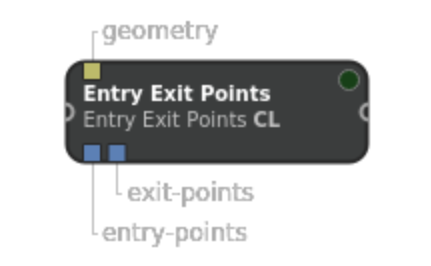
\includegraphics[width=1.00000\textwidth]{Images/processor.png}
\caption{Exempel på en processors utseende.}
\label{fig:Processor}
\end{figure}

De färgade rutorna till vänster på processorn i figur \ref{fig:Processor} är
olika typer av ingångar och utgångar. Cirkeln i det övre högra hörnet på
processorn i samma figur är en lampa som lyser då processorn är aktiv.
De processorer som ENVISIoN skapat kategoriseras och beskrivs nedan.

\subsubsection{Kristallstruktur}\label{kristallstruktur}

Nedanstående processorer är relaterade till visualiseringen av
kristallstrukturer. De tillhör en modul vid namn Crystalvisualization.

\textbf{CoordinateReader} Från en HDF5-fil läser denna processor
koordinater för atompositioner. En sökväg till ett dataset sätts via en
StringProperty path\_. I molekyldynamiksfall så används en tidstegsräknare IntProperty timestep\_ som varierar värdet som på path\_.
Utdata från CoordinateReader är \emph{n} stycken vec3.

Inport:

\begin{itemize}
\tightlist
\item
  Hdf5::Inport inport\_
\end{itemize}

Utport:

\begin{itemize}
\tightlist
\item
  DataOutport\textless{} std::vector\textless{}vec3\textgreater{}
  \textgreater{} outport\_
\end{itemize}

Properties:

\begin{itemize}
\tightlist
\item
  StringProperty path\_
\item 
  IntProperty timestep\_
\end{itemize}

\textbf{StructureMesh} Atompostionsdata kopplas ihop med rätt atomfärg
och radie med StructureMesh-processorn. StructureMesh har en
multiinport, dit en eller flera CoordinateReader-processorer kan kopplas
in. Indata för StructureMesh är atompositionsdata i form av vec3 för
varje atomslag. Till denna indata läggs properties för färg, radie och
antal till för varje atomslag/processor som kopplas in. Den ger en mesh,
som har buffrar för position, färg och radie.

Inport:

\begin{itemize}
\tightlist
\item
  DataInport\textless{} std::vector\textless{}vec3\textgreater{},
  0\textgreater{} structure\_
\end{itemize}

Utport:

\begin{itemize}
\tightlist
\item
  MeshOutport mesh\_
\end{itemize}

Properties:

\begin{itemize}
\tightlist
\item
  FloatProperty scalingFactor\_
\item
  FloatMat3Property basis\_
\item
  BoolProperty fullMesh\_
\item
  IntProperty timestep\_
\item
  std::vector\textless{}
  std::unique\_ptr\textless{}FloatVec4Property\textgreater{}
  \textgreater{} colors\_: vektor som innehåller färgproperty för varje
  atomslag
\item
  std::vector\textless{} std::unique\_ptr\textless{}FloatProperty
  \textgreater{} \textgreater{} radii\_: vektor som innehåller
  radieproperty för varje atomslag
\item
  std::vector\textless{}
  std::unique\_ptr\textless{}IntProperty\textgreater{} \textgreater{}
  num\_: vektor som innehåller antalet atomer per tidssteg för varje
  atomslag
\item
  BoolProperty enablePicking\_: sann då picking-funktionen är påslagen
\item
  IntVectorProperty inds\_: vektor med index på valda atomer
\end{itemize}

\subsubsection{HDF5}\label{hdf5}

Nedanstående processorer är ämnade att fungera väl med de
HDF5-relaterade processorer som är inkluderade i Inviwo.

\textbf{HDF5PathSelection*} Detta är en grupp av processorer som har
funktionalitet liknande den inbyggda processorn HDF5PathSelection. En
eller flera av dessa processorer placeras med fördel mellan en HDFSource
och en eller flera HDF5To*.

Gemensamt för dessa processorer är att de på inporten tar en Hdf5-grupp
och på utporten skriver noll eller flera av dessa omedelbara
undergrupper.

Nedan beskrivs de olika processorerna i denna grupp.

\textbf{HDFpathSelectionInt} Denna processor väljer en HDF5-grupp med
heltalsnamn, baserat på värdet på processorns intProperty\_, eventuellt
utökat med ledande nollor till bredden specificerat på processorns
zeroPadWidthProperty\_.

HDF5PathSelectionInt kan med fördel användas tillsammans med en
OrdinalPropertyAnimator för att plocka ut relevant data ur en HDF5-fil.

Anledningen till att utdata ges som en vektor av HDF5-grupper, trots att
processorn alltid skriver exakt en grupp på utporten, är att processorn
ska följa samma mönster som, och fungera väl med, resterande
processorer.

Inport:

\begin{itemize}
\tightlist
\item
  DataInport\textless{}hdf5::Handle\textgreater{} hdf5HandleInport\_
\end{itemize}

Utport:

\begin{itemize}
\tightlist
\item
  DataOutport\textless{}
  std::vector\textless{}hdf5::Handle\textgreater{} \textgreater{}
  hdf5HandleVectorOutport\_
\end{itemize}

Properties:

\begin{itemize}
\tightlist
\item
  IntProperty intProperty\_
\item
  IntSizeTProperty zeroPadWidthProperty\_
\end{itemize}

\textbf{HDF5PathSelectionIntVector} Denna processor väljer noll eller
flera HDF5-grupper med heltalsnamn, baserat på värdet på processorns
intVectorProperty\_, eventuellt utökat med ledande nollor till berdden
specificerat av processorns zeroPadWidthProperty\_.

HDF5PathSelectionIntVector kan med fördel användas tillsammans med
''picking'' för att plocka ut relevant data ur en HDF5-fil.

Inport:

\begin{itemize}
\tightlist
\item
  DataInport\textless{}hdf5::Handle\textgreater{} hdf5HandleInport\_
\end{itemize}

Utport:

\begin{itemize}
\tightlist
\item
  DataOutport\textless{}
  std::vector\textless{}hdf5::Handle\textgreater{} \textgreater{}
  hdf5HandleVectorOutport\_
\end{itemize}

Properties:

\begin{itemize}
\tightlist
\item
  IntVectorProperty intVectorProperty\_
\item
  IntSizeTProperty zeroPadWidthProperty\_
\end{itemize}

\textbf{HDF5PathSelectionAllChildren} Denna processor väljer den givna
HDF5-gruppens alla undergrupper.

Inport:

\begin{itemize}
\tightlist
\item
  DataInport\textless{}hdf5::Handle\textgreater{} hdf5HandleInport\_
\end{itemize}

\textbf{HDF5To*} Detta är en grupp av processorer som har funktionalitet
liknande den inbyggda processorn HDF5ToVolume. Processorerna placeras
med fördel efter en HDFSource-processor, med en eller flera mellan
liggande HDF5PathSelection*.

Gemensamt för dessa är att de som indata tar noll eller flera
HDF5-grupper (baserat på *pathSelectionProperty\_), plockar ut dataset
för varje grupp och omvandlar dessa till relevanta objekt (Point eller
Function) som sedan skrivs till utporten. Objektens variabel-metadata
tas, om de finns tillgängliga, från attributen associerade med
dataseten. Vidare kan, om så väljs med *namePrependParentsProperty\_,
metadat utökas med namnen på de grupper var i dataseten ligger.

Vilka dataset som kan väljas med *pathSelectionProperty\_ uppdateras
dynamiskt beroende på vilka grupper som ligger på inporten. När ett
lämpligt dataset valts kan *pathFreezeProperty\_ användas för att stänga
av denna dynamik, så att värdet sparas även om grupperna på inporten
(antagligen tillfälligt) ändras. Detta underlättar manuellt
experimenterande samt användandet av processorer som tillfälligt ger
noll grupper som utadat, t.ex. HDF5PathSelectionIntVector.

\textbf{HDF5ToPoint} Denna processor konverterar HDF5-data till noll
eller flera Point-objekt.

Inport:

\begin{itemize}
\tightlist
\item
  DataInport\textless{}hdf5::Handle, 0, true\textgreater{}
  hdf5HandleFlatMultiInport\_
\end{itemize}

Utport:

\begin{itemize}
\tightlist
\item
  DataOutport\textless{} std::vector\textless{}Point\textgreater{}
  \textgreater{} pointVectorOutport\_
\end{itemize}

Properties:

\begin{itemize}
\tightlist
\item
  OptionPropertyString pathSelectionProperty\_
\item
  BoolProperty pathFreezeProperty\_
\item
  IntSizeTProperty namePrependParentsProperty\_
\end{itemize}

\textbf{HDF5ToFunction} Denna processor konverterar HDF5-data till noll
eller flera Function-objekt.

Normalt plockas två dataset per grupp ut, ett för x-axeln och ett för
y-axeln. Om endast data för y-axeln finns tillgänglig kan
implicitXProperty\_ sättas, varvid processorn automatgenererar data för
x-axeln.

Inport:

\begin{itemize}
\tightlist
\item
  DataInport\textless{}hdf5::Handle, 0, true\textgreater{}
  hdf5HandleFlatMultiInport\_
\end{itemize}

Utport:

\begin{itemize}
\tightlist
\item
  DataOutport\textless{} std::vector\textless{}Function\textgreater{}
  \textgreater{} functionVectorOutport\_
\end{itemize}

Properties:

\begin{itemize}
\tightlist
\item
  BoolProperty implicitXProperty\_
\item
  OptionPropertyString xPathSelectionProperty\_
\item
  OptionPropertyString yPathSelectionProperty\_
\item
  BoolProperty xPathFreezeProperty\_
\item
  BoolProperty yPathFreezeProperty\_
\item
  IntSizeTProperty xNamePrependParentsProperty\_
\item
  IntSizeTProperty yNamePrependParentsProperty\_
\end{itemize}

\subsubsection{2D}\label{d}

Nedanstående processorer är ämnade att bearbeta och presentera 2D-data,
närmare bestämt data av typen Point och Function.

\textbf{FunctionOperationUnary} Denna processor implementerar en unär
operator, antingen negation \((g_{i}(x) = -f_{i}(x))\) eller
(multiplikativ) inversion \((g_{i}(x) = 1/f_{i}(x))\). Operatorn
appliceras på funktioner på inporten, en i taget, och skriver respektive
resultat på utporten.

Inport:

\begin{itemize}
\tightlist
\item
  DataFrameInport dataframeInport\_
\end{itemize}

Utport:

\begin{itemize}
\tightlist
\item
  DataFramOutport dataframOutport\_
\end{itemize}

Properties:

\begin{itemize}
\tightlist
\item
  OptionPropertyString operationProperty\_
\end{itemize}

\textbf{FunctionOperationNary} Denna processor implementerar en operator
med variabel aritet (engelska n-ary), antingen addition/summa
\((g(x) = \Sigma_{i}f_{i}(x))\) eller multiplikation/produkt
\((g(x) = \Pi_{i}f_{i}(x))\). Operatorn appliceras på samtliga
funktioner på inporten och skrver resultatet på utporten.

Då funktionerna på inporten kan vara samplade vid olika x-värden behöver
processorn ta beslut om var ut-funktionen ska samplas. Processorn utgår
från att sampla i samtliga x-värden för samtliga in-funktioner.
sampleFilterEnableProperty\_ kan sättas för att filtrera dessa. Då
sampleFilterEnableProperty\_ är satt ser processorn till att
sampelavståndet är minst det värde som anges i
sampleFilterEpsilonProperty\_. När processorn skapas är
sampleFilterEnableProperty\_ satt och sampleFilterEpsilonProperty\_ är 0
vilket innebär att x-värden som är identiska filtreras bort.

Om ett värde behöver beräknas vid ett x-värde där en in-funktion inte är
samplat används linjär interpolation om x-värdet ligger innanför
funktionens definitionsintervall. Om x-värdet ligger utanför detta
intervall används undefinedFallbackProperty\_ för att avgöra vilket
värde som används istället. Detta kan antingen vara noll eller
funktionens värde vid intervallets relevanta ändpunkt.

Inport

\begin{itemize}
\tightlist
\item
  org.envision.FunctionFlatMultiInport functionFlatMultiInport\_
\end{itemize}

Utport:

\begin{itemize}
\tightlist
\item
  DataFramOutport dataframOutport\_
\end{itemize}

Properties:

\begin{itemize}
\tightlist
\item
  OptionsPropertyString operationProperty\_
\item
  OptionsPropertyString undefinedFallbackProperty\_
\item
  BoolProperty sampleFilterEnableProperty\_
\item
  FloatProperty sampleFilterEpsilonProperty\_
\end{itemize}

\textbf{LinePlot} LinePlot tar en \emph{DataFrame} som förväntas
innehålla minst två kolumner med data. Den konstruerar en mesh som
representerar en linjegraf. Denna mesh renderas sedan, förslagsvis med
hjälp av en \emph{2D Mesh Renderer}-processor för att generera en bild
av grafen.

LinePlot genererar även en utbild att lägga över grafen som innehåller
axelgraderingen. Axelgraderingen kan också den skickas in i \emph{2D
Mesh Renderer}-processorn och kommer då läggas ovanpå grafen.

Användaren väljer vilken kolumn i den \emph{DataFrame} som processorn
tar in som ska representeras på vardera axel genom val i
\emph{xSelectionProperty\_} och \emph{ySelectionProperty\_}. Vill
användaren välja multipla kolumner som ska representeras på y-axeln
sätts \emph{boolYSelection\_} till sant för att sedan välja vilka
kolumner i med hjälp av en sträng i \emph{groupYSelection\_}. Användaren
kan även välja alla kolumner som inte representeras på x-axeln att
representeras på y-axeln genom att sätta \emph{allYSelection\_} till
sant.

Inställningar som har \emph{range} i namnet justerar minimum- och
maximumvärden på koordinataxlarna. Inställningar med \emph{width} eller
\emph{colour} justerar bredd respektive färg för olika linjer ritade i
diagrammet.

\emph{label\_number\_} anger antalet divisioner på koordinataxlarna. Är
värdet till exempel satt till tjugo innebär det att varje axel kommer ha
tjugo divisioner och tjugo axelgraderingsetiketter, utöver de etiketter
på startvärdena på vardera axel.

\emph{font\_} ställer in vilket typsnitt axelgraderingen skall ha.

\emph{enable\_line\_} aktiverar ritandet av en vertikal linje på
x-koordinaten specificerad i \emph{line\_x\_coordinate\_}. Denna är
avsedd att ge en visuell markering av var specifika x-värden finns på
x-axeln.

Inport:

\begin{itemize}
\tightlist
\item
  DataFrameInport dataFrameInport\_
\item
  DataInport\textless{}Point, 0, true\textgreater{} pointInport\_
\end{itemize}

Utports:

\begin{itemize}
\tightlist
\item
  MeshOutport meshOutport\_
\item
  ImageOutport labels\_
\end{itemize}

Properties:

\begin{itemize}
\tightlist
\item
  OptionPropertyString xSelectionProperty\_
\item
  OptionPropertyString ySelectionProperty\_
\item
  StringProperty groupYSelection\_
\item
  BoolProperty boolYSelection\_
\item
  BoolProperty allYSelection\_
\item
  FloatVec4Property colour\_
\item
  FloatVec2Property x\_range\_
\item
  FloatVec2Property y\_range\_
\item
  FloatProperty scale\_
\item
  BoolProperty enable\_line\_
\item
  FloatProperty line\_x\_coordinate\_
\item
  FloatVec4Property line\_colour\_
\item
  BoolProperty show\_x\_labels\_
\item
  BoolProperty show\_y\_labels\_
\item
  FloatVec4Property axis\_colour\_
\item
  FloatProperty axis\_width\_
\item
  BoolProperty enable\_grid\_
\item
  FloatVec4Property grid\_colour\_
\item
  FloatProperty grid\_width\_
\item
  FontProperty font\_
\item
  FloatVec4Property text\_colour\_
\item
  IntProperty label\_number\_
\end{itemize}

\textbf{DataFrameCollector}\\
Processorn utför inga beräkningar, utan den samlar endast ihop DataFrame
från ett godtyckligt antal andra processorer till endast en DataFrame.
Behovet för denna processor dök upp då visualiseringen för
tillståndstäthet uppdaterades. Önskan att välja specifika partiella
tillstånd kunde uppfyllas med hjälp av denna processor.

Inport:

\begin{itemize}
\tightlist
\item
  DataInport\textless{}DataFrame, 0\textgreater{} dataframeInport\_
\end{itemize}

Utport:

\begin{itemize}
\tightlist
\item
  DataFrameOutport dataframeOutport\_
\end{itemize}

\textbf{FunctionToDataFrame}\\
Denna processor extraherar data från funktioner till en DataFrame där
varje funktion ger upphov till två kolumner. All data i en funktion har
även information om densamma, t.ex. variabelnamn och enhet. Namnet på
vardera kolumn som skapas är dess variabelnamn från funktionen.

Processorn skapades då det tidigare inte funnits ett sätt att extrahera
data från flera funktioner samtidigt. Då har lösningen varit att använda
en processor för varje funktion som har data att extrahera.
Problematiken med den lösningen är att en visualisering kan vara väldigt
tidskrävande. En visualisering av bandstruktur kan potentiellt ha flera
hundra funktioner. Med FunctionToDataFrame kan detta göras med endast en
processor.

Inport:

\begin{itemize}
\tightlist
\item
  DataInport\textless{}Function, 0, true\textgreater{}
  functionFlatMultiInport\_
\end{itemize}

Utport:

\begin{itemize}
\tightlist
\item
  DataFrameOutport dataframeOutport\_
\end{itemize}

\subsubsection{Fermi}\label{fermi}

\textbf{HDF5FermiSource}

Process used for reading HDF5 data pertaining to fermi surface data

Outport:

\begin{quote}
\begin{description}
\item[volumeOutport: ivw.data.VolumeOutport]
Final processed data
\end{description}
\end{quote}

Properties:

\begin{quote}
\begin{description}
\item[energy\_band: ivw.properties.IntProperty]
Specifiees the band that should be read from the HDF5 file
\item[is\_brillouin\_zone: ivw.propertiesBoolProperty]
Specifies if the data should be translated to birllouin zone
\item[is\_expanded\_zone: ivw.propertiesBoolProperty]
Specifies if the data should be translated to expanded zone. Note if
is\_brillouin\_zone is set this property will be overriden
\end{description}
\end{quote}

\begin{description}
\item[\textbf{\_\_init\_\_(self, id, name):}]
\begin{description}
\item[id: str]
ID given to the process
\item[name: str]
name given to the process
\end{description}
\item[\textbf{brillouin\_zone(self, matrix, basis)}]
Transforms reciprocal lattice to brillouin zone

\begin{description}
\item[Parameters:]
\begin{description}
\item[matrix: numpy.array]
3D Matrix should represent reciprocal lattice
\item[basis:]
Reciprocal basis vectors
\end{description}
\item[Return:]
Matrix representing the brillouin zone
\end{description}
\item[\textbf{expanded\_zone(self, matrix)}]
Expands given matrix 4 quadrents

\begin{description}
\item[Parameters:]
\begin{description}
\item[matrix: numpy.array]
3D Matrix should represent reciprocal lattice
\end{description}
\item[Return:]
Expanded matrix
\end{description}
\item[\textbf{process(self, matrix, basis)}]
Reads hdf\_file set in self.filename, normalises the data and translates
it to an \emph{Inviwo-Volum}

Additional options to expand the data and to translate the data to
brillouin zone are possible through the \emph{Inviwo-properties}

\begin{description}
\item[Returns:]
None
\end{description}
\end{description}

\subsubsection{Molekyldynamik}\label{Molekyldynamik}
\textbf{Property Animator}
För animeringen av Molekyldynamik används processorn Property Animator. Processorn ändrar en \emph{property} hos en annan processor över tiden.

Först måste en property skapas i processorn. Denna property är någon form av taltyp t.ex. ett float-tal eller en interger. Propertyn har ett \emph{value} som är dess siffervärde och ett värde kallat \emph{delta} som bestämmer hur snabbt \emph{value} förändras med tiden. Förändring av \emph{value} med tiden initieras av att trycka \emph{play}-knappen i property Animator. \emph{Value} kan länkas till en property hos en annan processor. Detta gör att propertyn i denna processor sätts till värdet som \emph{value} har. När \emph{value} förändras av \emph{delta} förändras även den property som \emph{value} är länkat till.

\subsection{Properties och widgets}\label{properties-och-widgets}

\subsubsection{IntVectorpropety}\label{intvectorpropety}

Denna property består av en vektor av int-värden.

\subsubsection{IntVectorPropertyWidget}\label{intvectorpropertywidget}

En widget för IntVectorProperty. ''Textbox'', satt till endast läsning
(read only), som innehåller de värden som finns i tillhörande
IntVectorProperty.

\newpage
\section{Envisionpy}\label{envisionpy}

ENVISIoNs pythonkod ligger i en modul kallad envisionpy. Det är i denna
som all pythonfunktionalitet som diskuteras i andra kapitel ligger.
Modulen har skapats för att man relativt enkelt ska kunna importera
ENVISIoNs funktionalitet från ett annat godtyckligt pythonskript
(exempelvis som det används i det senare beskrivna GUI-systemet \cite{GUI}).

Envisionpy har två undermappar, \emph{processor\_network} och
\emph{hdf5parser}. I dessa ligger de pythonfiler som beskrivs i \ref{networkhandlers}
respektive \ref{parsersystemet}. Den har även en undermapp
\emph{utils} där speciella Exception-klasser och fil med atomdata
ligger.

\subsection{EnvisionMain}\label{envisionmain}

Envisionpy har en klass kallad \emph{EnvisionMain}. Denna klass har som
uppgift att bilda ett gränssnitt som annan pythonkod kan styra all
ENVISIoNs visualiserings- och parsningsfunktionalitet från. När ett
\emph{EnvisionMain}-objekt initieras så startar denna sin egen instans
av Inviwo, med hjälp utav \emph{inviwopyapp}, som den kör i bakgrunden.
Detta tillåter att Inviwos visualiseringsfunktionalitet används utan att
dess gränssnitt visas.

\emph{EnvisionMain} kan genom funktionsanrop köra parsning och starta
ett godtyckligt antal visualiseringar genom att initera
\emph{NetworkHandler}-klasser allternativt \emph{Subnetwork}-klasser beroende på vilken visualisering som ska köras.

Alla \emph{NetworkHandler}-objekt sparas i en dictionary,
\emph{networkHandlers}, under en speciell identifikations-sträng som
specificeras då objektet initieras.

De funktioner som primärt används i EnvisionMain är
\emph{handle\_request} och \emph{parse\_vasp}. Det är
via dessa funktioner som parsnings- och visualiseringssystemen styrs. Det finns även en funktion parse\_ELK som används vid inläsning av ELK-filer.

\subsubsection{handle\_request}\label{handle_request}
För att påverka visualiseringarna så används
\emph{handle\_request}-funktionen. Denna tar ett argument kallat
\emph{request}. \emph{request} en lista på följande form :

{[}ACTION, HANDLER\_ID, {[}PARAMETERS\ldots{}{]}{]}.

ACTION är en sträng som beskriver vilken funktion som ska köras. En
dictionary, \emph{action\_dict}, finns som översätter olika strängar
till funktioner.

HANDLER\_ID ska innehålla en identifikationssträng för det
\emph{NetworkHandler}-objekt/\emph{Subnetwor}-objekt  som funktionen ska köras på. Om en ny
visualisering ska startas så specificerar den id för det nya
\emph{NetworkHandler}-objekt/\emph{Subnetwor}-objekt  som kommer att skapas.

{[}PARAMETERS\ldots{}{]} är en lista av parametrar som den specificerade
funktionen ska kallas med.

Funktionen returnerar en lista på följande form:

{[}ACTION, STATUS, HANDLER\_ID, RESPONSE\_DATA{]} där:

ACTION och HANDLER\_ID är samma strängar som funktionen tog emot.

STATUS är en bool som signalerar om funktionen lyckades eller
misslyckades.

RESPONSE\_DATA är någon godtycklig data som funktionen som körts har
returnerat, sätts till \emph{None} om ingen data returneras.

\subsubsection{parse\_vasp}\label{handle_parse_request}

För att köra parsningsfunktioner för inläsning av filer från VASP körs funktionen parse\_VASP. Funktionen tar in tre argument på följande form:\\

parse\_VASP(VASP\_path, hdf5\_path, parse\_types)\\ 

VASP\_path är en sträng som signalerar var data ska läsas ifrån, hdf5\_path är en sträng som specificerar var hdf5 filen ska sparas och parse\_types antingen är en  lista  med  strängar  som  signalerar  vilka parsningstyper som ska utföras eller strängen "All" för att inikera att alla parstyper ska köras.

\subsubsection{parse\_ELK}
För att köra parsningsfunktioner för inläsning av filer från ELK körs funktionen parse\_ELK. Funktionen tar in tre argument på följande form:\\

parse\_ELK(ELK\_path, hdf5\_path, parse\_types)\\ 

ELK\_path är en sträng som signalerar var data ska läsas ifrån, hdf5\_path är en sträng som specificerar var hdf5 filen ska sparas och parse\_types antingen är en  lista  med  strängar  som  signalerar  vilka parsningstyper som ska utföras eller strängen "All" för att inikera att alla parstyper ska köras.
\newpage
\section{ENVISIoN GUI}\label{gui}
Det grafiska gränssnittet har utvecklats för att underlätta körningen av de flesta visualisering som ENVISIoN tillåter. Genom att köra Inviwo i bakgrunden kan användaren få tillgång till de inställningarna som anses relevanta för visualiseringen i fråga. 

GUI:t är skrivet i Python och använder sig av paketet PySimpleGUI för att generera de grafiska elementen. 

\subsection{Kommunikation med envisionpy}
GUI:t är uppbyggt så att alla förfrågningar gällande visualiseringar skickas via de EnvisionMain funktioner som beskrivs i \ref{envisionmain}.

\subsection{Utseende}
När GUI.py skriptet körs öppnas GUI.
\begin{figure}[H]
\centering
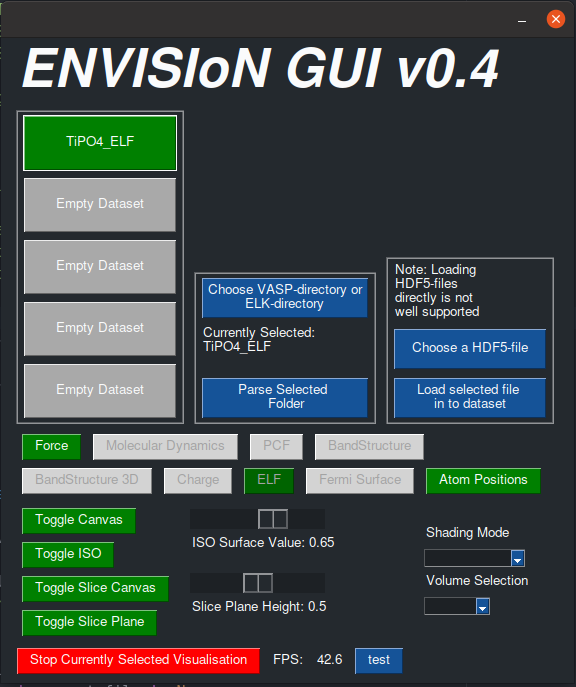
\includegraphics[width=0.70000\textwidth]{Images/gui_look.PNG}
\caption{Utseende på GUI.}
\label{fig:Gui_look}
\end{figure}

\newpage
\section{ENVISIoN Legacy GUI}\label{gui-systemet}

Här följer information om ENVISIoNs gamla GUI.

Det grafiska användargränssnittet har skapats för att underlätta
användandet av ENVISIoN. GUI:t möjliggör att ENVISIoN kan köras utan att
öppna Inviwos användarfönster.

GUI:t är utvecklat som en websida och körs med hjälp utav Electron.
Gränssnittet är skrivet med HTML, CSS, och JavaScript.

\subsection{Kommunukation med
envisionpy}\label{kommunukation-med-envisionpy}

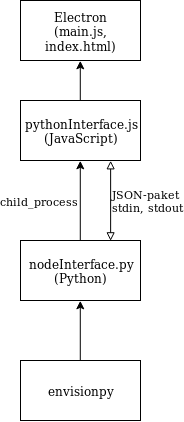
\includegraphics[width=0.30000\textwidth]{Images/gui-system-structure.png}

\emph{Skiss över GUI-systemet}

För att GUI-systemet ska kunna använda sig av envisionpy så används
nodemodulen \emph{child\_process}. \emph{child\_process} tillåter att
man från JavaScript startar en pythonprocess som kör ett specificerat
skript.

För att kommunicera mellan processerna så kan python-processens stdin
och stdout användas. JavaScript- och Python-processerna skickar
JSON-objekt kodade som strängar på detta sätt. När ett JSON-paket tas
emot så parsas det och funktioner körs beroende på innehållet. Detta görs i filerna \emph{pythonInterface.js} och
\emph{nodeInterface.py}.

Från JavaScript så startas en \emph{child\_process} som kör
pythonskriptet \emph{nodeInterface.py}. Detta skript sätter upp
kommunikationen med JavaScript och initierar en instans av
envisionpy.EnvisionMain.

\subsubsection{JSON-paket specifikation}\label{json-paket-specifikation}

JSON-objekten som skickas via stdin och stdout från och till python är
på följande form:

\{tag: TAG\_STRING, data: DATA\} där

TAG\_STRING: Är en sträng som specificerar vad datapaketet har att göra
med. I nuläget så används följande taggar. \emph{``envision request''}
då en visualisering ska påverkas. \emph{``parse request''} då parsning
ska utföras. \emph{``response''} då paketet innehåller svarsinformation
om en utförd funktion.

DATA är någon godtycklig data. Exakt vad den innehåller varierar stort.

\subsection{Utseende}\label{utseende}

När ENVISIoN-applikationen körs öppnas det grafiska gränssnittet.

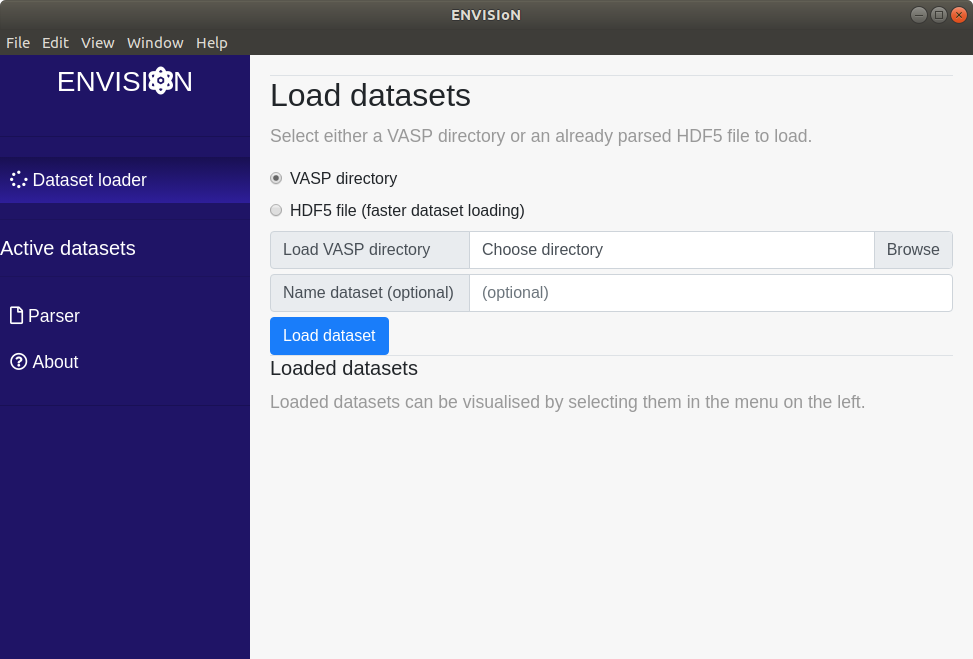
\includegraphics[width=0.60000\textwidth]{Images/GUI_start_Ubuntu.png}

\emph{GUI utseende vid start i Linux}

\newpage
\section{Referenser}\label{referenser}

\begin{thebibliography}{9}
 \bibitem{Inviwo} \href{https://inviwo.org/}{Inviwo} (hämtad 2019-05-10)

 \bibitem{API} \href{https://www.ne.se/uppslagsverk/encyklopedi/lång/api-(data)}{API}  (hämtad 2019-05-16)

 \bibitem{BSD2} \href{https://opensource.org/licenses/BSD-2-Clause}{BSD2}  (hämtad 2019-05-10)

 \bibitem{Cpp}\href{http://www.cplusplus.com/info/description/}{C++} (hämtad 2019-01-28).

 \bibitem{dict} \href{https://docs.python.org/3/tutorial/datastructures.html}{Data Structures}  (hämtad 2019-05-17).

\bibitem{Fermi-energi} Solid State Physics, Neil Ashcroft och David Mermin, 1976, s. 141.

\bibitem{Git}  \href{https://git-scm.com}{Git} (hämtad 2019-01-28).

\bibitem{GUI} \href{https://www.ne.se/uppslagsverk/encyklopedi/lång/api-(data)}{GUI} (hämtad 2019-05-10)

\bibitem{HowToUseHDF5FilesinPython}  \href{https://www.pythonforthelab.com/blog/how-to-use-hdf5-files-in-python/}{How To Use HDF5 Files in Python} (hämtad 2019-02-26).

\bibitem{Molekyldynamik} \href{https://www.ne.se/uppslagsverk/encyklopedi/lång/molekyldynamik}{Molekyldynamik} (hämtad 2021-04-19)

\bibitem{Python}  \href{https://www.python.org/}{Python} (hämtad 2019-01-28)

\bibitem{Python3}  \href{https://docs.python.org/3/}{Python3} (hämtad 2019-05-10)

\bibitem{PyQT} \href{https://www.riverbankcomputing.com/static/Docs/PyQt5/}{PyQT} (hämtad 2019-05-16)

\bibitem{WhatIsArray}  \href{https://www.programiz.com/python-programming/array\#introduction}{Python Arrays} (hämtad 2019-05-21).

\bibitem{WhatIsUNIX}  \href{https://www.softwaretestinghelp.com/unix-introduction/}{What is UNIX?} (hämtad 2019-05-21).

\bibitem{wxPython}  \href{https://wxpython.org/pages/overview/}{wxPython} (hämtad 2019-05-16)

\bibitem{wxPythonDoc}  \href{https://docs.wxpython.org/wx.1moduleindex.html}{wxPython Documentation} (hämtad 2019-05-17)

\bibitem{QuickStartGuide}  \href{http://docs.h5py.org/en/stable/quick.html\#appendix-creating-a-file}{Quick Start Guide} (hämtad 2019-02-26).

\bibitem{RadialDistributionFunction}  \href{https://en.wikipedia.org/wiki/Radial\distribution\function}{Radial distribution function}, , (hämtad 2019-03-03).

\bibitem{HDFGroup} \href{https://support.hdfgroup.org/HDF5/}{The HDF Group, Hierarchical Data Format, version 5 1997-2019} (hämtad 2018-01-28).

\bibitem{HDFGroup2}  \href{https://support.hdfgroup.org/HDF5/Tutor/HDF5Intro.pdf}{The HDF Group. High Level Introduction to HDF5. 23 Sept. 2016} (hämtad 2019-01-28).

\bibitem{Unittest}  \href{https://docs.python.org/3/library/unittest.html}{Unittest} (hämtad 2019-03-06).

\bibitem{VASP}  \href{https://www.vasp.at/index.php/about-vasp/59-about-vasp}{VASP} (hämtad 2019-02-26).


\end{thebibliography}


\newpage
\section{Appendix A - ENVISIoNs
HDF5-filstruktur}\label{appendix-a---envisions-hdf5-filstruktur}

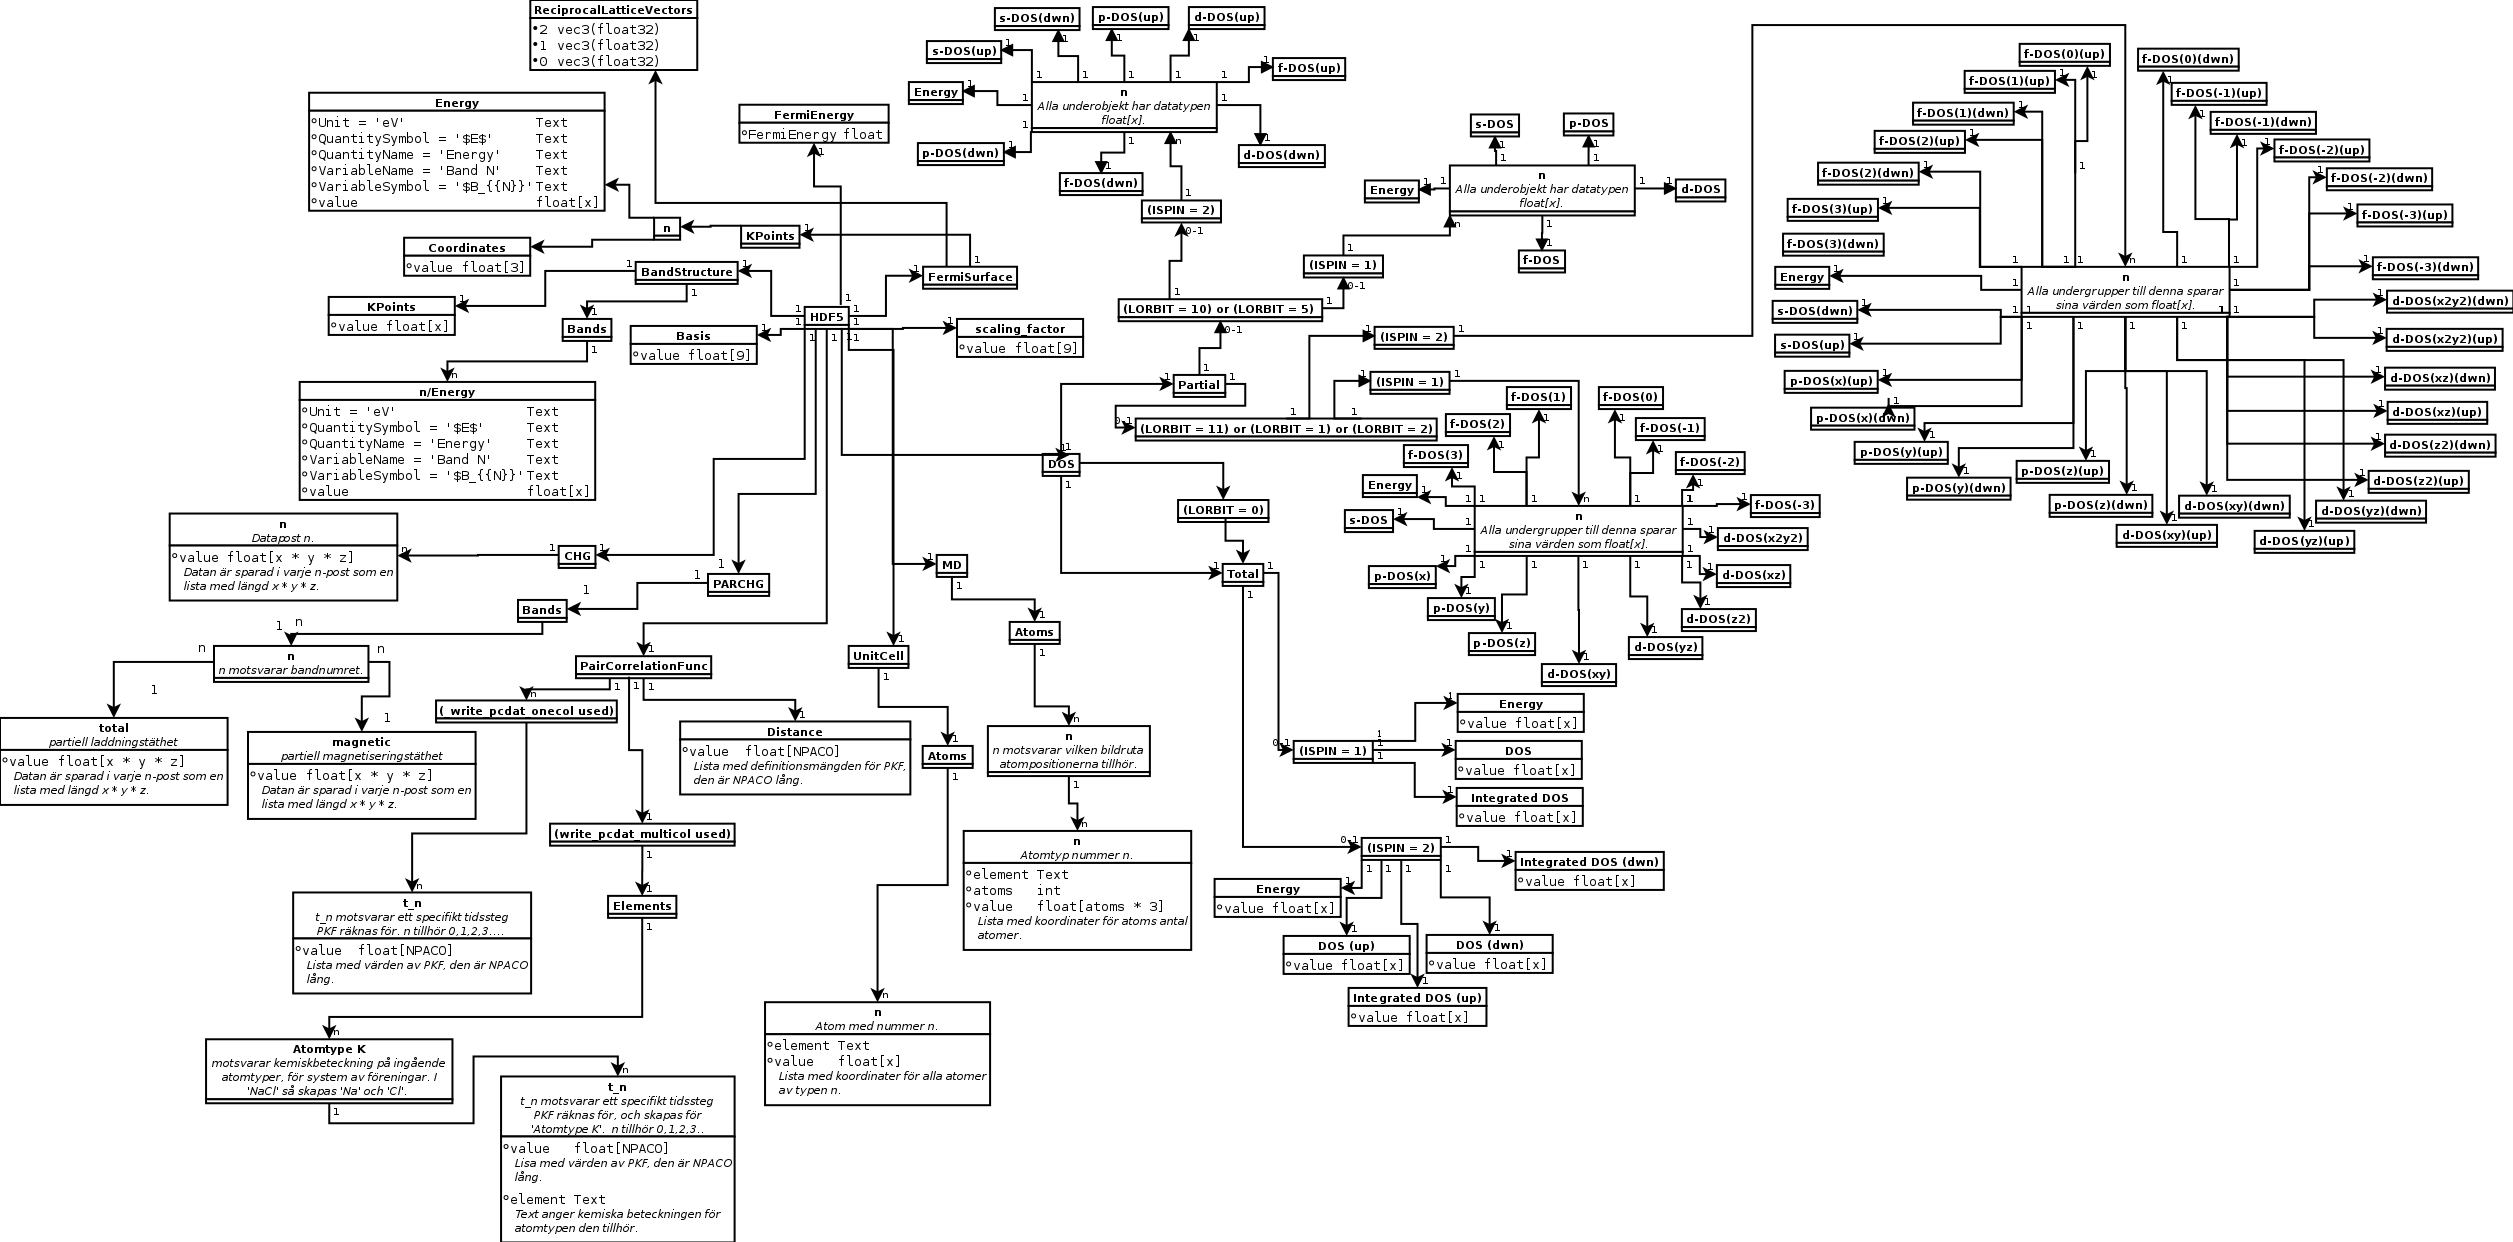
\includegraphics[width=1.00000\textwidth]{Images/UPDATE-hdf5-dataformat3modi.png}

\end{document}
